%%%% -*- Mode: LaTeX -*-
%!TEX encoding = UTF-8 Unicode

% =====================================================================
% Central Limit Theorem Report
% =====================================================================

%\documentclass[12pt,fleqn]{book}
\documentclass[oneside,onecolumn,12pt,a4paper,openany]{report}

\usepackage[notindex]{tocbibind}

\usepackage[square,numbers]{natbib}
\bibliographystyle{abbrvnat}

\usepackage[T1]{fontenc}
\usepackage[utf8]{inputenc}

\usepackage{amsmath}
\usepackage{amssymb}
%\usepackage{amsbsy}
\usepackage{amsthm}
\usepackage{bbm} % for \mathbbm{1}
\usepackage{imakeidx}
\usepackage{alltt}
\usepackage{holtexbasic}
\usepackage{LaTeX/layout}
\usepackage{graphicx}
\usepackage{LaTeX/proof}
\usepackage{supertabular}
\usepackage{url}
\usepackage{fancyvrb}
\usepackage[format=hang,justification=raggedright]{caption}  % multi-line figure caption

\hyphenation{docu-ments}
\newtheorem{theorem}{Theorem}[section]
\newtheorem{corollary}{Corollary}[theorem]
\newtheorem{lemma}[theorem]{Lemma}
\theoremstyle{remark}
\newtheorem*{remark}{Remark}
\newtheorem{proposition}[theorem]{Proposition}

% ---------------------------------------------------------------------
% Input defined macros and commands
% ---------------------------------------------------------------------
% =====================================================================
%
% Macros for typesetting the HOL system manual
%
% =====================================================================

% ---------------------------------------------------------------------
% Abbreviations for words and phrases
% ---------------------------------------------------------------------

\newcommand\TUTORIAL{{\footnotesize\sl TUTORIAL}}
\newcommand\DESCRIPTION{{\footnotesize\sl DESCRIPTION}}
\newcommand\REFERENCE{{\footnotesize\sl REFERENCE}}
\newcommand\LOGIC{{\footnotesize\sl LOGIC}}
\newcommand\LIBRARIES{{\footnotesize\sl LIBRARIES}}
\usepackage{textcomp}

\newcommand{\bs}{\texttt{\char'134}} % backslash
\newcommand{\lb}{\texttt{\char'173}} % left brace
\newcommand{\rb}{\texttt{\char'175}} % right brace
\newcommand{\td}{\texttt{\char'176}} % tilde
\newcommand{\lt}{\texttt{\char'74}} % less than
\newcommand{\gt}{\texttt{\char'76}} % greater than
\newcommand{\dol}{\texttt{\char'44}} % dollar
\newcommand{\pipe}{\texttt{\char'174}}
\newcommand{\apost}{\texttt{\textquotesingle}}
% back quote (tt font)
\newcommand{\bq}{\texttt{\char'140}}
% double back quotes ``
\newcommand{\dq}{\bq\bq}
% "fancy" versions of the same
\newcommand{\fldq}{\mbox{\textrm{\textquotedblleft}}}
\newcommand{\frdq}{\mbox{\textrm{\textquotedblright}}}
\newcommand{\fholquote}[1]{\fldq#1\frdq}
\newcommand{\ldquo}{\mbox{\textrm{``}}}
\newcommand{\rdquo}{\mbox{\textrm{''}}}
\newcommand{\lsquo}{\mbox{\textrm{`}}}
\newcommand{\rsquo}{\mbox{\textrm{'}}}

%These macros were included by slind:

\newcommand{\holquote}[1]{\dq#1\dq}
\newcommand{\uholquote}[1]{\mbox{\rmfamily\upshape ``}#1\mbox{\rmfamily\upshape ''}}

\def\HOL{\textsc{Hol}}
\def\holn{\HOL}  % i.e. hol n(inety-eight), no digits in
                 % macro names is a bit of a pain; deciding to do away
                 % with hol98 nomenclature means that we just want to
                 % write HOL for hol98.
\def\holnversion{Trindemossen-1}
\def\holnsversion{Trindemossen~1} % version with space rather than hyphen
\def\LCF{{\small LCF}}
\def\LCFLSM{{\small LCF{\kern-.2em}{\normalsize\_}{\kern0.1em}LSM}}
\def\PPL{{\small PP}{\kern-.095em}$\lambda$}
\def\PPLAMBDA{{\small PPLAMBDA}}
\def\ML{{\small ML}}
\def\holmake{\texttt{Holmake}}

\newcommand\ie{\mbox{\textit{i{.}e{.}}}}
\newcommand\eg{\mbox{\textit{e{.}g{.}}}}
\newcommand\viz{\mbox{viz{.}}}
\newcommand\adhoc{\mbox{\it ad hoc}}
\newcommand\etal{{\it et al.\/}}
% NOTE: \etc produces wrong spacing if used between sentences, that is
% like here \etc End such sentences with non-macro etc.
\newcommand\etc{\mbox{\textit{etc{.}}}}

% ---------------------------------------------------------------------
% Simple abbreviations and macros for mathematical typesetting
% ---------------------------------------------------------------------

\newcommand\fun{{\to}}
\newcommand\prd{{\times}}

\newcommand\conj{\ \wedge\ }
\newcommand\disj{\ \vee\ }
\newcommand\imp{ \Rightarrow }
\newcommand\eqv{\ \equiv\ }
\newcommand\cond{\rightarrow}
\newcommand\vbar{\mid}
\newcommand\turn{\ \vdash\ } % FIXME: "\ " results in extra space
\newcommand\hilbert{\varepsilon}
\providecommand\eqdef{\ \equiv\ }
\renewcommand\eqdef{\ \equiv\ }

\newcommand\natnums{\mbox{${\sf N}\!\!\!\!{\sf N}$}}
\newcommand\bools{\mbox{${\sf T}\!\!\!\!{\sf T}$}}

\newcommand\p{$\prime$}
\newcommand\f{$\forall$\ }
\newcommand\e{$\exists$\ }

\newcommand\orr{$\vee$\ }
\newcommand\negg{$\neg$\ }

\newcommand\arrr{$\rightarrow$}
\newcommand\hex{$\sharp $}

\newcommand{\uquant}[1]{\forall #1.\ }
\newcommand{\equant}[1]{\exists #1.\ }
\newcommand{\hquant}[1]{\hilbert #1.\ }
\newcommand{\iquant}[1]{\exists ! #1.\ }
\newcommand{\lquant}[1]{\lambda #1.\ }

\newcommand{\leave}[1]{\\[#1]\noindent}
\newcommand\entails{\mbox{\rule{.3mm}{4mm}\rule[2mm]{.2in}{.3mm}}}

% ---------------------------------------------------------------------
% Font-changing commands
% ---------------------------------------------------------------------

\newcommand{\theory}[1]{\hbox{{\small\tt #1}}}
\newcommand{\theoryimp}[1]{\texttt{#1}}

\newcommand{\con}[1]{{\sf #1}}
\newcommand{\rul}[1]{{\tt #1}}
\newcommand{\ty}[1]{\textsl{#1}}

\newcommand{\ml}[1]{\mbox{{\def\_{\char'137}\texttt{#1}}}}
\newcommand{\holtxt}[1]{\ml{#1}}
\newcommand\ms{\tt}
\newcommand{\s}[1]{{\small #1}}

\newcommand{\pin}[1]{{\bf #1}}
% FIXME: for multichar symbols \mathit should be used.
\def\m#1{\mbox{\normalsize$#1$}}

% ---------------------------------------------------------------------
% Abbreviations for particular mathematical constants etc.
% ---------------------------------------------------------------------

\providecommand{\T}{\con{T}}
\renewcommand{\T}{\con{T}}
\newcommand\F{\con{F}}
\newcommand\OneOne{\con{One\_One}}
\newcommand\OntoSubset{\con{Onto\_Subset}}
\newcommand\Onto{\con{Onto}}
\newcommand\TyDef{\con{Type\_Definition}}
\newcommand\Inv{\con{Inv}}
\newcommand\com{\con{o}}
\newcommand\Id{\con{I}}
\newcommand\MkPair{\con{Mk\_Pair}}
\newcommand\IsPair{\con{Is\_Pair}}
\newcommand\Fst{\con{Fst}}
\newcommand\Snd{\con{Snd}}
\newcommand\Suc{\con{Suc}}
\newcommand\Nil{\con{Nil}}
\newcommand\Cons{\con{Cons}}
\newcommand\Hd{\con{Hd}}
\newcommand\Tl{\con{Tl}}
\newcommand\Null{\con{Null}}
\newcommand\ListPrimRec{\con{List\_Prim\_Rec}}


\newcommand\SimpRec{\con{Simp\_Rec}}
\newcommand\SimpRecRel{\con{Simp\_Rec\_Rel}}
\newcommand\SimpRecFun{\con{Simp\_Rec\_Fun}}
\newcommand\PrimRec{\con{Prim\_Rec}}
\newcommand\PrimRecRel{\con{Prim\_Rec\_Rel}}
\newcommand\PrimRecFun{\con{Prim\_Rec\_Fun}}

\newcommand\bool{\ty{bool}}
\newcommand\num{\ty{num}}
\newcommand\ind{\ty{ind}}
\newcommand\lst{\ty{list}}

% ---------------------------------------------------------------------
% \minipagewidth = \textwidth minus 1.02 em
% ---------------------------------------------------------------------

\newlength{\minipagewidth}
\setlength{\minipagewidth}{\textwidth}
\addtolength{\minipagewidth}{-1.02em}

% ---------------------------------------------------------------------
% Environment for the items on the title page of a case study
% ---------------------------------------------------------------------

\newenvironment{inset}[1]{\noindent{\large\bf #1}\begin{list}%
{}{\setlength{\leftmargin}{\parindent}%
\setlength{\topsep}{-.1in}}\item }{\end{list}\vskip .4in}

% ---------------------------------------------------------------------
% Macros for little HOL sessions displayed in boxes.
%
% Usage: (1) \setcounter{sessioncount}{1} resets the session counter
%
%        (2) \begin{session}\begin{verbatim}
%             .
%              < lines from hol session >
%             .
%            \end{verbatim}\end{session}
%
%            typesets the session in a numbered box.
% ---------------------------------------------------------------------

\newlength{\hsbw}
\setlength{\hsbw}{\textwidth}
\addtolength{\hsbw}{-\arrayrulewidth}
\addtolength{\hsbw}{-\tabcolsep}
\newcommand\HOLSpacing{13pt}

\newcounter{sessioncount}
\setcounter{sessioncount}{0}

\newenvironment{session}{\begin{flushleft}
 \refstepcounter{sessioncount}
 \begin{tabular}{@{}|c@{}|@{}}\hline
 \begin{minipage}[b]{\hsbw}
 \vspace*{-.5pt}
 \begin{flushright}
 \rule{0.01in}{.15in}\rule{0.3in}{0.01in}\hspace{-0.35in}
 \raisebox{0.04in}{\makebox[0.3in][c]{\footnotesize\sl \thesessioncount}}
 \end{flushright}
 \vspace*{-.55in}
 \begingroup\small\baselineskip\HOLSpacing}{\endgroup\end{minipage}\\ \hline
 \end{tabular}
 \end{flushleft}}

% ---------------------------------------------------------------------
% Macro for boxed ML functions, etc.
%
% Usage: (1) \begin{holboxed}\begin{verbatim}
%               .
%               < lines giving names and types of mk functions >
%               .
%            \end{verbatim}\end{holboxed}
%
%            typesets the given lines in a box.
%
%            Conventions: lines are left-aligned under the "g" of begin,
%            and used to highlight primary reference for the ml function(s)
%            that appear in the box.
% ---------------------------------------------------------------------

\newenvironment{holboxed}{\begin{flushleft}
  \begin{tabular}{@{}|c@{}|@{}}\hline
  \begin{minipage}[b]{\hsbw}
% \vspace*{-.55in}
  \vspace*{.06in}
  \begingroup\small\baselineskip\HOLSpacing}{\endgroup\end{minipage}\\ \hline
  \end{tabular}
  \end{flushleft}}

% ---------------------------------------------------------------------
% Macro for unboxed ML functions, etc.
%
% Usage: (1) \begin{hol}\begin{verbatim}
%               .
%               < lines giving names and types of mk functions >
%               .
%            \end{verbatim}\end{hol}
%
%            typesets the given lines exactly like {boxed}, except there's
%            no box.
%
%            Conventions: lines are left-aligned under the "g" of begin,
%            and used to display ML code in verbatim, left aligned.
% ---------------------------------------------------------------------

\newenvironment{hol}{\begin{flushleft}
 \begin{tabular}{c@{}@{}}
 \begin{minipage}[b]{\hsbw}
% \vspace*{-.55in}
 \vspace*{.06in}
 \begingroup\small\baselineskip\HOLSpacing}{\endgroup\end{minipage}\\
 \end{tabular}
 \end{flushleft}}

% ---------------------------------------------------------------------
% Emphatic brackets
% ---------------------------------------------------------------------

\newcommand\leb{\lbrack\!\lbrack}
\newcommand\reb{\rbrack\!\rbrack}


% ---------------------------------------------------------------------
% Quotations
% ---------------------------------------------------------------------


%These macros were included by ap; they are used in Chapters 9 and 10
%of the HOL DESCRIPTION

\newcommand{\inds}%standard infinite set
 {\mbox{\rm I}}

\newcommand{\ch}%standard choice function
 {\mbox{\rm ch}}

\newcommand{\den}[1]%denotational brackets
 {[\![#1]\!]}

\newcommand{\two}%standard 2-element set
 {\mbox{\rm 2}}


\usepackage{scalerel}
\usepackage[only,llbracket,rrbracket,llparenthesis,rrparenthesis]{stmaryrd}
\parskip 1ex
\parindent 0ex
\usepackage{accsupp} % for ensuring the right Unicode codepoint upon pasting

\newcommand*{\llbrace}{%
  \BeginAccSupp{method=hex,unicode,ActualText=2983}%
    \textnormal{\usefont{OMS}{lmr}{m}{n}\char102}%
    \mathchoice{\mkern-4.05mu}{\mkern-4.05mu}{\mkern-4.3mu}{\mkern-4.8mu}%
    \textnormal{\usefont{OMS}{lmr}{m}{n}\char106}%
  \EndAccSupp{}%
}
\newcommand*{\rrbrace}{%
  \BeginAccSupp{method=hex,unicode,ActualText=2984}%
    \textnormal{\usefont{OMS}{lmr}{m}{n}\char106}%
    \mathchoice{\mkern-4.05mu}{\mkern-4.05mu}{\mkern-4.3mu}{\mkern-4.8mu}%
    \textnormal{\usefont{OMS}{lmr}{m}{n}\char103}%
  \EndAccSupp{}%
}


%\includeonly{title,contents,preface,ML,logic,semantics,system,drules,conv,see}

%\includeonly{title,contents,preface,ML,logic,semantics,system,drules,conv,index,see}
%\includeonly{title,contents,preface,ML}
%\includeonly{tactics}
%\includeonly{preface,ack}
%\includeonly{logic,semantics}
%\includeonly{system,theories,libraries}

%\usepackage[hidelinks,hypertexnames=false]{hyperref}
%\hypersetup{
%  pdftitle={CLT Report},
%  pdfauthor={Kai Phan},
%  pdfsubject={HOL4},
%  pdfkeywords={Interactive Theorem Proving; Higher Order Logic},
%  pdfdisplaydoctitle=true
%}

\usepackage{breakurl} % it depends on hyperref

\usepackage{centernot}
\newcommand{\notiff}{\nLeftrightarrow}

\theoremstyle{definition}
\newtheorem{definition}[equation]{Definition}


\makeindex[intoc]
\begin{document}

   \setlength{\unitlength}{1mm}           % unit of length = 1mm
   \setlength{\baselineskip}{16pt}        % line spacing = 16pt

   % ---------------------------------------------------------------------
   % prelims
   % ---------------------------------------------------------------------

%   \pagenumbering{roman}                  % roman page numbers for prelims
%   \setcounter{page}{1}                   % start at page 1

   % %%%% -*- Mode: LaTeX -*-
% %!TEX encoding = UTF-8 Unicode

%\crefformat{footnote}{#2\footnotemark[#1]#3}
%\usepackage{sidecap}
%\renewcommand{\bottomfraction}{0.7}

\newcommand{\thesistitle}{Formal Verification of Central Limit Theorem}
\newcommand{\thesistitletwo}{in HOL Theorem Prover}
\newcommand{\thesistitlethree}{  }
\newcommand{\fullname}{Thi Cam Tu Phan}
\newcommand{\shortname}{Kai Phan}
\newcommand{\thesissubjects}{Probability Theory, HOL4, Interactive Theorem Proving, Proof Mechanisation}
\newcommand{\thesisdate}{May 2025}
\newcommand{\fullthesisdate}{\today}
\newcommand{\resubmissiondate}{\today}
\newcommand{\thesisyear}{2025}


% epigraph settings, for quotes at the start of introduction and conclusions
%\setlength{\epigraphwidth}{12cm}
%\setlength{\afterepigraphskip}{1.5cm}
%\renewcommand{\epigraphsize}{\small}
%\renewcommand{\epigraphrule}{1pt}
%\renewcommand{\epigraphflush}{flushright}
%\renewcommand{\textflush}{flushleft}
%\citestyle{aa}
\pagestyle{empty}

%
%%% TITLE PAGE:
\pagenumbering{arabic}  % first use Roman numerals for page numbers

\begin{titlepage}
  \begin{center}
    \vspace*{0cm}
    { \fontsize{20}{10} \selectfont \thesistitle} \\
    \vspace{0.3cm}
    { \fontsize{20}{10} \selectfont \thesistitletwo} \\
            \vspace{0.3cm}
    { \fontsize{20}{10} \selectfont \thesistitlethree}

    \vspace{1.75cm}
    {\bf \huge \fullname}\\
    %\vfill
    \vspace{1.75cm}
    {\large A thesis submitted for the degree of}\\
    \vspace{0.5cm}
    {\it \large Master of Computing (Advanced)}\\
    \vspace{0.5cm}
    {\large The Australian National University}\\
    \vspace{0.5cm}
    { \large School of Computing} \par
    \vspace{0.5cm}
    {\large Supervisor: Dr. Chun Tian}\\
    \vspace{2.0cm}
    
\includegraphics[width=0.4\textwidth]{anu-logo-colour.pdf}\\
    \vspace{2.0cm}
    {\large \thesisdate}

    % {\bf Submitted:}\\
    %{\bf Approved:}\\
    \vspace{1.5cm}
    {\large  \textcopyright\ Copyright by \fullname,  \thesisyear \\}
    \vspace{0.5cm}
    {\large All Rights Reserved}
        %\maketitle
  \end{center}
\end{titlepage}
                        % description title page
   \chapter*{Abstract}
\label{abstract}

This thesis presents a formalisation of Lyapunov’s Central Limit Theorem (CLT) in the HOL4 theorem prover. The proof follows the Lindeberg replacement method and employs Taylor expansion techniques to quantify the difference between the distribution of normalised partial sums and the standard normal distribution.

The formalisation enriches HOL4’s existing \texttt{ProbabilityTheory} by introducing additional infrastructure necessary for the proof, including higher-order derivatives, bounds on smooth functions, and properties of moment conditions.

A key outcome of this work is a modular and rigorous development of the Lindeberg-based proof of the CLT, which complements existing formal efforts in \texttt{ProbabilityTheory} in HOL4. The approach demonstrates that classical analytical techniques can be accurately mechanised using modern theorem proving tools.
                      % preface to entire description
%   \chapter*{Acknowledgements}\markboth{Acknowledgements}{Acknowledgements}

The bulk of \HOL\ is based on code written by---in alphabetical
order---%
Hasan Amjad,
Richard Boulton,
Anthony Fox,
Mike Gordon,
Elsa Gunter,
John Harrison,
Peter Homeier,
G\'erard Huet (and others at INRIA),
Joe Hurd,
Ramana Kumar,
Ken Friis Larsen,
Tom Melham,
Robin Milner,
Lockwood Morris,
Magnus Myreen,
Malcolm Newey,
Michael Norrish,
Larry Paulson,
Konrad Slind,
Don Syme,
Chun Tian,
Thomas T\"urk,
Chris Wadsworth,
and
Tjark Weber.
Many others have supplied parts of the system, bug fixes, etc.

\subsection*{Current edition}

The current edition of all four volumes (\LOGIC, \TUTORIAL,
\DESCRIPTION\ and \REFERENCE) has been prepared by Michael Norrish and
Konrad Slind. Further contributions to these volumes came from: Hasan
Amjad, who developed a model checking library and wrote sections
describing its use; Jens Brandt, who developed and documented a
library for the rational numbers; Anthony Fox, who formalized and
documented new word theories and the associated libraries; Mike
Gordon, who documented the libraries for BDDs and SAT; Peter Homeier,
who implemented and documented the quotient library; Joe Hurd, who
added material on first order proof search; Chun Tian, who documented the HOL theories for probability and measure theory; and Tjark Weber, who wrote
libraries for Satisfiability Modulo Theories~(SMT) and Quantified
Boolean Formulae~(QBF).

\medskip

The material in the third edition constitutes a thorough re-working
and extension of previous editions.  The only essentially unaltered
piece is the semantics by Andy Pitts (in \LOGIC), reflecting the fact
that, although the \HOL\ system has undergone continual development
and improvement, the \HOL\ logic is unchanged since the first edition
(1988).

\newpage

\subsection*{Second edition}

The second edition of \REFERENCE\ was a joint effort by the Cambridge
\HOL\ group.

\subsection*{First edition}

The three volumes \TUTORIAL, \DESCRIPTION\ and \REFERENCE\ were
produced at the Cambridge Research Center of SRI International with
the support of DSTO Australia.

The \HOL\ documentation project was managed by Mike Gordon, who also
wrote parts of \DESCRIPTION\ and \TUTORIAL\ using material based on an
early paper describing the \HOL\ system\footnote{M.J.C.\ Gordon, `HOL:
  a Proof Generating System for Higher Order Logic', in: {\it VLSI
    Specification, Verification and Synthesis\/}, edited by G.\
  Birtwistle and P.A.\ Subrahmanyam, (Kluwer Academic Publishers,
  1988), pp.\ 73--128.} and {\sl The ML Handbook\/}\footnote{{\sl The
    ML Handbook}, unpublished report from Inria by Guy Cousineau, Mike
  Gordon, G\'erard Huet, Robin Milner, Larry Paulson and Chris
  Wadsworth.}.  Other contributers to \DESCRIPTION\ incude Avra Cohn,
who contributed material on theorems, rules, conversions and tactics,
and also composed the index (which was typeset by Juanito Camilleri);
Tom Melham, who wrote the sections describing type definitions, the
concrete type package and the `resolution' tactics; and Andy Pitts,
who devised the set-theoretic semantics of the \HOL\ logic and wrote
the material describing it.

The original document design used \LaTeX\ macros supplied by Elsa
Gunter, Tom Melham and Larry Paulson.  The typesetting of all three
volumes was managed by Tom Melham.  The cover design is by Arnold
Smith, who used a photograph of a `snow watching lantern' taken by
Avra Cohn (in whose garden the original object resides).  John Van
Tassel composed the \LaTeX\ picture of the lantern.

Many people other than those listed above have contributed to the
\HOL\ documentation effort, either by providing material, or by
sending lists of errors in the first edition.  Thanks to everyone who
helped, and thanks to DSTO and SRI for their generous support.

\newpage
\subsection*{In Memory of Mike Gordon}

As documented in the academic literature, in material available from his archived web-pages at the University of Cambridge Computer Laboratory, and in these manuals, Mike Gordon was \HOL's primary creator and developer.
Mike not only created a significant piece of software, inspiring this and many other projects since, but also built a world-leading research group in the Computer Laboratory.
This research environment was wonderfully productive for many of the system's authors, and we all owe Mike an enormous debt for both the original work on \HOL, and for the way he and his group supported our own development as researchers and \HOL{} hackers.

\bigskip
\begin{center}
Mike Gordon, 1948--2017
\end{center}
                   % global acknowledgements
   \tableofcontents                       % table of contents


%   \cleardoublepage
%   \pagenumbering{arabic}                % arabic page numbers
%   \setcounter{page}{1}                  % start at page 1

%   \include{draft}
   \chapter[Introduction]{Introduction}
\label{chap:1}

The idea of a formalised mechanist is simple but powerful: to trust mathematics in software, we must mechanise not only calculations but also proofs. A mechanist builds a logic engine where every theorem arises from a small set of primitive rules. If those rules are sound, everything derived from them inherits that soundness.

HOL4 supports this mechanised philosophy \cite{slind2008brief}. It encodes logic using a typed \(\lambda\)-calculus and restricts theorem creation to a protected MetaLanguage (ML) type, ensuring that every step is checked with mathematical rigour.

This thesis formalises one of the most fundamental results in probability theory: the Central Limit Theorem (CLT). When many independent effects accumulate, their combined influence often resembles a bell curve. The CLT explains this universal phenomenon observed across diverse fields—from biology and economics to physics and computation.

We focus on Lyapunov’s version of the CLT as presented in Chung~\cite{Chung:2001}, using Lindeberg’s replacement method.


\medskip
\noindent
\textbf{The Central Limit Theorem (Lyapunov form):}
\begin{quote}
Let \( \{X_i\} \) be a sequence of independent real-valued random variables defined over a probability space \( p \), with the following properties:
\begin{itemize}
  \item Each \( X_i \) has mean zero: \( \mathbb{E}[X_i] = 0 \);
  \item Each \( X_i \) has finite, non-zero variance: \( 0 < \text{Var}(X_i) < \infty \);
  \item Each \( X_i \) has finite third absolute moment: \( \mathbb{E}[|X_i|^3] < \infty \);
  \item The sequence \( X_i \) is independent in the formal sense used in HOL4 (via \texttt{indep\_vars} over Borel sets).
\end{itemize}

Define the sum \( S_n = \sum_{i=0}^{n-1} X_i \), and let the total variance be \( s_n^2 = \sum_{i=0}^{n-1} \text{Var}(X_i) \).

If the Lyapunov condition holds:
\[
\frac{\sum_{i=0}^{n-1} \mathbb{E}[|X_i|^3]}{s_n^3} \to 0 \quad \text{as } n \to \infty,
\]
then the normalised sum converges in distribution to the standard normal:
\[
\frac{S_n}{s_n} \xrightarrow{d} \mathcal{N}(0,1).
\]
\end{quote}

In HOL4, we express this formally as:

\begin{center}
\scriptsize
\begin{hol}
\begin{alltt}
Theorem central\_limit\_theorem :
\(\!\!\!{\turn}\!\!\!\!\) \(\forall\)p X N.
prob\_space p \(\land\)
ext\_normal\_rv N p 0 1 \(\land\)
(\(\forall\)i. real\_random\_variable (X i) p) \(\land\)
(\(\forall\)n. indep\_vars p X (\(\lambda\)i. Borel) (count n)) \(\land\)
(\(\forall\)i. expectation p (X i) = 0) \(\land\)
(\(\forall\)i. expectation p (\(\lambda\)x. (abs (X i x))\(^3\)) < \(+\infty\)) \(\land\)
(\(\forall\)i. variance p (X i) < PosInf) \(\land\)
(\(\forall\)i. variance p (X i) \(\ne\) 0) \(\land\)
(\(\forall\)n. (sqrt (second\_moments p X n)) \(\ne\) 0) \(\land\)
((\(\lambda\)n. (third\_moments p X n) / ((sqrt (second\_moments p X n)) pow 3)) --> 0) sequentially
\(\Rightarrow\)
((\(\lambda\)n x. (SIGMA (\(\lambda\)i. X i x) (count n)) / (sqrt (second\_moments p X n))) --> N)
(in\_distribution p)
\end{alltt}
\end{hol}
\end{center}

Although the final convergence result is not yet complete, this work marks a significant advance toward a fully formalised CLT. Over 6000 lines of HOL4 code were written, including formal definitions, measure-theoretic infrastructure, Taylor approximations, moment bounds, and Big-O analysis.

An initial attempt to follow the moment-generating function route was abandoned due to limited HOL4 support for improper integrals and Laplace transforms. The current approach, based on Taylor expansions and the Lindeberg method, allowed all core analytic steps to be formalised. The only missing component involves evaluating the third absolute moment of the normal distribution, which requires gamma-function integrals not yet formalised in HOL4.

This remaining gap is technical, not conceptual. Once suitable analysis tools become available, the full convergence proof can be completed with minimal additional effort.

   %%% -*- Mode: LaTeX; -*-

\chapter[Background and Related Work]{Background and Related Work}
\label{chap:2}



% \section{Background and Related Work}
% \textbf{Purpose:} Position this work in the context of previous efforts and provide foundational concepts.
% \subsection{Overview of the Central Limit Theorem}
% \begin{itemize}
%     \item Explain the statement of the CLT and its generalizations (e.g., Lyapunov’s and Lindeberg’s approaches).
%     \item Focus on Lyapunov’s version as the basis of this proof:

%      \begin{equation}
%      \text{If } \frac{\Gamma_n}{s_n^3} \to 0 \text{ as } \space \space n \to \infty,
%      \end{equation}
%      then
%      \[
%      \frac{S_n}{s_n} \xrightarrow{d} \Phi.
%      \]
%      Define key terms: \( \Gamma_n, s_n, S_n \), and Lyapunov’s condition.
% \end{itemize}

The Central Limit Theory is one of the main theoretical results from the  Probability theory, a bridge from individual randomness to aggregate predictability. It marks the gradual approach of mathematical rigor and upgrading of the theorem used by addressing more and more difficult problems. Over centuries, different forms of CLTs have been derived, each of which has added to its understanding convergence and applications. This chapter will present the historical development of the CLT that describes its milestones and contributions. It will also examine the modern theorem proving tools and ways of formalization, focusing on Lyapunov's approach.

\section{Historical Background}
Let us just trace briefly the historical evolution of the CLT, critical milestones, key contributors, and the gradual refinement of its conditions and scope. The roots of the CLT go back to the dispute of the eighteenth century, specifically to the time Abraham de Moivre laid the foundation for this theorem. In 1733, de Moivre showed that the sum of a large number of independent and identically distributed random variables converges to the normal distribution-an elegant approximation to problems such as the rolling of dice or repeated coin flips \cite{de1733approximatio}. His work initiated the interplay between discrete distributions-such as the Binomial-and their continuous approximations, and laid the ground for developments to come.

In 1810, Pierre-Simon Laplace independently extended de Moivre's insights by proving a much more general form of this theorem. Under broader conditions, Laplace demonstrated convergence of the sum of independent random variables to a normal distribution, thereby establishing CLT as a universal principle. His work was used in applying the CLT to population statistics and measurement errors \cite{laplace1835oeuvres} and cemented its usefulness for aggregate phenomena analysis.

The 19th century would see the formalization of the central limit theorem (CLT) by Pafnuty Chebyshev, who also gave the theorem a rigorous foundation by the introduction of variance and expectation conditions. With that work, Chebyshev rendered the CLT mathematically precise, linking it to the developing area of probability theory \cite{chebyshev1890deux}. Building on this work was further advancing the generalization of the CLT by Alexander Lyapunov to sequences of independent random variables that are not identically distributed. His version of the theorem brought forth Lyapunov's condition, which contained definite criteria for convergence \cite{lyapunov1895pafnutii}.

In the early years of the 20th century, contributions by Lyapunov represented such a change in the evolution of the CLT. Unlike his predecessors, Lyapunov sought a “direct” and “elementary” proof. It would try to make the theorem internal relations simpler and relax the theorem's assumptions. His papers published in 1900 and 1901 reconstructed previous methods with a rigor of Weierstrass, and introduced new precision to the theorem by establishing explicit bounds on the normalized sum and the limiting normal distribution. This specificity answers Chebyshev's earlier demand for sharper probabilistic results although it should have simplified the proof through some clever but much deeper refinements of Poisson's arguments \cite{fischer2011history}.

Lyapunov’s goals extended beyond mere generalization; he aimed to illuminate the theorem’s internal structure and make it more accessible. Avoiding the complexities of characteristic functions and complex analysis, he focused on moment-based criteria, relying on real-valued tools like Taylor expansions, bounding techniques, and Lyapunov's inequality. Thus the balance here is theoretical rigor and practical applicability, two characteristics that still resonate well with modern efforts at formal verification as that undertaken in this thesis.

In contemporary times, further refinements of the CLT were provided by William Feller bringing it to discrete random variables \cite{feller1945}, and all subsequent developments that are probabilistic have been geared towards this common extension to stable distributions and higher dimensional data. These extensions demonstrate the theorem’s adaptability to various contexts, from stochastic processes to machine learning and data analysis.

Lyapunov’s version of the CLT represents a key milestone in this journey. It generalizes the theorem for independent random variables with finite moments so that it becomes an observed but pliant frame of reference for convergence. It is this balancing between abstractness and concreteness that is a characteristic of the whole development of probability during the modern period. Contemporaries of Lyapunov such as von Mises, Lévy, Cramér, Khinchin, and Kolmogorov likewise pursued abstract relations in probability theory while keeping an eye on practical relevance. This tension is paradigmatically present in Lyapunov's work, which illustrates the way in which results which are purely formal mathematics may nonetheless satisfy external criteria of applicability and utility. For more information about the history and the proofs of the Central Limit Theorem, see \cite{fischer2011history, adams2009life}.

This thesis is based on the generalization of CLT as expressed in Lyapunov's version. Because of its focus on real-valued methods and moment-based criteria, it avoids any complex tools like characteristic functions or complex analysis, hence being particularly suitable for formalization in HOL4. In this respect, Lyapunov's approach not only advances the mathematical generalization but also provides a practical framework to meet the rigor and accessibility requirements of automated reasoning systems by directly addressing convergence under relaxed conditions.

\section{Related Work}

Formalization of mathematical theorems as proofs has been a singular research focus in modern computational mathematics. The systems such as Isabelle/HOL \citep{isabelle}, Coq \citep{bertot2013interactive}, and HOL4 \citep{slind2008brief} have been heavily relied on over the years to encode and prove basic properties but offer several features and challenges.

One of the most significant achievements in this area was the formalization of CLT within the Isabelle/HOL proof assistant. This was made possible mainly by the rich library related to complex analysis in Isabelle/HOL, which provided the means to make use of characteristic functions within the proof. Characteristic functions are Fourier transforms of probability distributions that make convergence easier to analyze by drawing on their special mathematical properties. Central to the approach are two key steps: first, pointwise convergence of the characteristic function for the normalized sum of independent random variables to that of the standard normal distribution should be demonstrated; and second, by the application of the L\'evy Continuity Theorem, one obtains the desired convergence in distribution. These two steps are actually the core of the proof that eventually leads to the verification of CLT \cite{billingsley2017probability}.

The characteristic function approach is beautifully complemented by the infrastructure provided by Isabelle/HOL, which supports careful manipulation of complex-valued functions, differentiation, and limits. This thereby enables Isabelle/HOL to achieve the rigorous performance that is demanded by Fourier analysis and probability theory. Among the striking personalities behind this effort is Luke Serafin, who has produced a giant leap forward in the formalization of the CLT \cite{serafin2015formally}. Serafin's systematic encoding of the characteristic function method has ensured that it was entirely generic and modular. His contributions involved the formalization of key intermediate results such as the for sums of independent random variables and the fact that components of his work are reusable, enabling extension into applications that relate to probabilistic theorems.

The strength of Isabelle/HOL is to borrow from its excellent complex analysis library. The characteristic function-based proofs are formalized smoothly, and the modular and extensible framework allows researchers to always build on previous work, gradually increasing the scope of formalized mathematics. The CLT formalization within Isabelle/HOL is exemplary in showing how even the most intricate probabilistic results can be encoded rigorously with the help of proof assistants. But this also points to some of the challenges with this approach: it is very much based on Fourier transforms and complex-valued methods, an infrastructure which may not always be as easily available when moving to other proof systems. Also, characteristic functions are powerful but often complicate proofs in situations where simpler real-valued methods, such as those based on moments, would suffice.

The formalization of CLT in Isabelle/HOL serves as an inspiration and comparison for the research presented in this thesis. The Example of Isabelle/HOL shows that the CLT can be formalized with the help of characteristic functions but also brings into relief the limitations of such a strategy-if proof assistants like HOL4 lack libraries comparable for complex analysis with it. This thesis takes a different site following the approach with the theorem of Lyapunov, which involves real-valued moment conditions rather than characteristic functions. Following this path, the work in HOL4 demonstrates how easier and less convoluted tools enable formulating the CLT while considering the inherent challenges of formal verification.

   %%% -*- Mode: LaTeX; -*-
\chapter[Preliminaries]{Preliminaries}
\label{chap:3}

This chapter describes an overview of the theoretical and formal theories required for the formalization of the Central Limit Theorem . This includes HOL Formalization, Measure Theory, Lebesgue Integration, and Probability Theory.
\section{HOL Formalization}
Higher Order Logic (HOL) \cite{hol4, slind2008brief} is derived from the Logic of Computable Functions (LCF) \cite{gordon1979edinburgh, milner1972logic} created by Robin Milner and colleagues in 1972. HOL is an adaptation of Church's Simple Theory of Types (STT) \cite{church1940formulation}, where a higher-order version of Hilbert's choice operator \(\varepsilon \), Axiom of Infinity, and Rank-1 polymorphism have been added. HOL4 implements the original HOL framework, while other theorem provers in the HOL family, such as Isabelle/HOL, include important extensions. Such a simple logical basis makes HOL more accessible than those systems founded on much more advanced dependent type theories, such such the Calculus of Inductive and Co-Inductive Constructions constructed by Coq. Therefore, theories and proofs founded on HOL are easier for a layman to comprehend rather than being lost in a complicated type theory.

HOL refers both to the logical system and the software implementing it. HOL4 is the latest version of this software and written in Standard ML (SML), a general-purpose functional programming language.  SML has played the most vital role in the HOL4 for implementing its core engine, enabled automation due to which proof tactics have been written in that and also for interaction, whether it is through a proof script or in direct correspondence with the user. Integrated SML gives a way in which HOL4 is versatile and can easily be extended such that complex verification tools are provided to develop the management of proofs by a user efficiently.

HOL terms are representatives of such things and the grammar includes constants, variables, applications (function calls) and lambda abstractions. Quantifiers, for instance universal (!x. P(x)) and existential (?x. P(x)), are also provided in HOL - they are defined as specific lambda functions.

The type system of HOL establishes the structural framework within which all terms and expressions are guaranteed to be well-defined and logically consistent. Types in HOL denote sets within the universe \( U \), and every term bears a certain type. The type grammar is simple and very expressive, and thus able to construct a wide variety of mathematical and logical objects.

The type grammar is defined as:
\[
\sigma ::= \alpha \ | \ c \ | \ (\sigma_1, \ldots, \sigma_n)\text{op} \ | \ \sigma_1 \to \sigma_2
\]
where:
\begin{enumerate}
    \item \textbf{Type Variables (\(\alpha, \beta, \ldots\)):} Generic placeholders that allow polymorphism to provide functions and predicates over different types.
    \begin{itemize}
        \item Example: The type variable \(\alpha\) could indicate integers, Booleans, or functions.
    \end{itemize}

    \item \textbf{Atomic Types (\(c\)):} Fixed and pre-defined types within HOL. The two initial atomic types are:
    \begin{itemize}
        \item \texttt{bool}: The set of Boolean values \(\{T, F\}\).
        \item \texttt{ind}: The set composed by individuals (an infinite set).

    \end{itemize}

    \item \textbf{Compound Types (\((\sigma_1, \ldots, \sigma_n)\text{op}\)):} Formed by applying type operators to other types. Their examples include Cartesian products, which designate the tuples over the elements.
    \begin{itemize}
        \item Example: The type \((\texttt{bool}, \texttt{ind}) \times\) represents pairs of a Boolean and an individual.
    \end{itemize}

    \item \textbf{Function Types (\(\sigma_1 \to \sigma_2\)):} Represent total functions mapping elements from a domain (\(\sigma_1\)) to a codomain (\(\sigma_2\)).
    \begin{itemize}
        \item Example: The type \(\texttt{bool} \to \texttt{ind}\) indicates a function mapping both Boolean-values to individual-elements.
    \end{itemize}
\end{enumerate}

For example, consider the following types:
\begin{enumerate}
    \item A function from integers to Booleans:
   \[
   f : \texttt{int} \to \texttt{bool}
   \]
   This type indicates that \(f(x)\) is a function taking an integer \(x\) and returning a Boolean.

    \item A tuple containing a Boolean and a function:
       \[
       p : (\texttt{bool}, (\texttt{int} \to \texttt{bool}))
       \]
       This is a pair type \(p = (b, f)\), where \(b\) is a Boolean, and \(f\) is a function mapping integers to Booleans.
       \item The type system guarantees the consistency by making sure all terms are properly typed. So if \(g : \texttt{int} \to \texttt{bool}\), then \(g(5)\) as 5 is an integer, but, \(g(T)\) would be invalid since \(T\) is a Boolean, not an integer. Such stringent typing is at the level of terms to avoid self-contradictory values and assure that proofs built up in HOL are sound.
\end{enumerate}

In HOL, terms are representatives for elements of sets represented by their types. The grammar of the term defines the syntax and structure for the logical expressions that can be expressed and hence statements that could be well typed and logically valid. Terms in HOL are constructed from the following components:

\[
t ::= x \ | \ c \ | \ t \ t' \ | \ \lambda x. t
\]
where:
\begin{enumerate}
\item \textbf{Variables} $\boldsymbol{(x, y, \ldots)}:$
    \begin{itemize}
        \item Represent placeholders for elements of a type.
        \item Example: \(x : \texttt{bool}\) stands for a Boolean variable.
    \end{itemize}

    \item \textbf{Constants (\(c\)):}
    \begin{itemize}
        \item Fixed entities such as \(T\), \(F\), mathematical operators, or predefined functions.
        \item  Example: The constant \(+\) defines addition for numeric types.
    \end{itemize}

   \item \textbf{Function Applications (\(t \ t'\)):}
   \begin{itemize}
       \item Define the application of a function to an argument. The term \(f(x)\) applies the function \(f\) to the variable \(x\).
        \item Example: If \(f : \texttt{int} \to \texttt{real}\) and \(x : \texttt{int}\), then \(f(x)\) is a valid term of type \(\texttt{real}\).
   \end{itemize}

\item \textbf{\(\lambda\)-Abstractions (\(\lambda x. t\)):}
\begin{itemize}
    \item Denote anonymous functions where \(x\) is the input variable, and \(t\) is the function body.
    \item Example: \(\lambda x. x + 1\) defines a function that increments its input by 1.
\end{itemize}


\end{enumerate}

To ensure consistency, the terms of HOL should be well typed. Given a term \(t_{\sigma}\) of type \(\sigma\), its grammar can be generalized with type annotations:

\[
t_{\sigma} ::= x_{\sigma} \ | \ c_{\sigma} \ | \ (t_{\sigma_1 \to \sigma_2} \ t'_{\sigma_1})_{\sigma_2} \ | \ (\lambda x_{\sigma_1}. t_{\sigma_2})_{\sigma_1 \to \sigma_2}
\]

HOL's deductive system is considered the logical foundation for forming and checking a proof. HOL's deductive system may consist of eight primitive rules of inference, the definition of new theorems by existing theorems. These rules are the basic components and are required for all logical reasoning within HOL, ensuring that proofs are consistent, logically valid, and traced. The following are the eight main primitive inference rules in HOL:

\begin{enumerate}
    \item \textbf{Assumption Introduction (ASSUME):}
    \begin{itemize}
        \item Introduces a formula as an assumption.
        \item Rule:
          \begin{center}
            \begin{tabular}{c}
              \\ \hline
              $t${\small\verb+ |- +}$t$ \\
            \end{tabular}
          \end{center}
        \item Example: From the assumption \(P\), we conclude \(P\).
    \end{itemize}

    \item \textbf{Reflexivity (REFL):}
    \begin{itemize}
        \item States that any term is equal to itself.
        \item Rule:
          \begin{center}
            \begin{tabular}{c}
              \\ \hline
                 {\small\verb+ |- +}$t${\small\verb+ = +}$t$ \\
            \end{tabular}
          \end{center}
        \item Example: For \(x : \texttt{int}\), \(x = x\) is always true.
    \end{itemize}

    \item \textbf{Beta Conversion (BETA\_CONV):}
    \begin{itemize}
        \item Applies substitution in lambda abstractions.
        \item Rule:
        \item Example: \((\lambda x. x + 1)(5) \vdash 5 + 1\).
    \end{itemize}

    \item \textbf{Substitution (SUBST):}
    \begin{itemize}
        \item Replaces a term in a formula with another term proven to be equal.
        \item Rule:
          \begin{center}
            \begin{tabular}{c}
              $\Gamma_1${\small\verb+ |- +} $t_1${\small\verb+=+}$t'_1$ {\small\verb+  +} $\cdots$ {\small\verb+  +}
              $\Gamma_n${\small\verb+ |- +} $t_n${\small\verb+=+}$t'_n$ {\small\verb+  +}
              $\Gamma${\small\verb+ |- +} $t[t_1,\ldots,t_n]$ \\ \hline
              $\Gamma_1 \cup \cdots
              \cup \Gamma_n \cup \Gamma${\small\verb+ |- +} $t[t'_1,\ldots,t'_n]$ \\
            \end{tabular}
          \end{center}
        \item Example: From \(x = y\) and \(P(x)\), infer \(P(y)\).
    \end{itemize}

    \item \textbf{Abstraction (ABS):}
    \begin{itemize}
        \item Generalizes an equation by abstracting a variable.
        \item Rule:
          \begin{center}
            \begin{tabular}{c}
              $\Gamma${\small\verb+ |- +}$t_1${\small\verb+ = +}$t_2$ \\ \hline
              $\Gamma${\small\verb+ |- (\+}$x${\small\verb+.+}$t_1${\small\verb+) = (\+}$x${\small\verb+.+}$t_2${\small\verb+)+} \\
            \end{tabular}
          \end{center}
        \item Example: From \(5 + 1 = 6\), infer \(\lambda x. x + 1 = \lambda x. 6\).
    \end{itemize}

    \item \textbf{Type Instantiation (INST\_TYPE):}
    \begin{itemize}
        \item Specializes polymorphic functions or predicates to specific types.
        \item Rule:
          \begin{center}
            \begin{tabular}{c}
              $\Gamma${\small\verb+ |- +}$t$ \\ \hline
              $\Gamma[\sigma_1,\ \ldots\ ,\sigma_n/\alpha_1,\ \ldots\ ,\alpha_n]${\small\verb+ |- +}$t[\sigma_1,\ \ldots\ ,\sigma_n/\alpha_1,\ \ldots\ ,\alpha_n]$
            \end{tabular}
          \end{center}
    \end{itemize}

    \item \textbf{Discharging Assumptions (DISCH):}
    \begin{itemize}
        \item Converts an assumption into an implication.
        \item Rule:
          \begin{center}
            \begin{tabular}{c}
              $\Gamma${\small\verb+ |- +} $t_2$ \\ \hline
              $\Gamma{-}\{t_1\}${\small\verb+ |- +} $t_1${\small\verb+ ==> +}$t_2$
            \end{tabular}
          \end{center}
        \item Example: From \(P \wedge Q\), infer \(P \Rightarrow (Q \wedge P)\).
    \end{itemize}

    \item \textbf{Modus Ponens (MP):}
    \begin{itemize}
        \item Combines an implication and its premise to infer the conclusion.
        \item Rule:
          \begin{center}
            \begin{tabular}{c}
              $\Gamma_1${\small\verb+ |- +}$t_1${\small\verb+ ==> +}$t_2$ {\small\verb+     +} $\Gamma_2${\small\verb+ |- +}$t_1$ \\
              \hline
              $\Gamma_1 \cup \Gamma_2${\small\verb+ |- +}$t_2$ \\
            \end{tabular}
          \end{center}
        \item Example: From \(x > 0 \Rightarrow x^2 > 0\) and \(x > 0\), infer \(x^2 > 0\).
    \end{itemize}
\end{enumerate}
These inference rules ensure that all logical derivations are traceable to basic axioms and established theorems. Additionally, the deductive system forms the backbone of HOL4, ensuring that proofs are both rigorous and reliable.

All proofs in HOL are fundamentally derived from a set of primitive inference rules and a core logical foundation. These rules define the semantics of two fundamental logical connectives: \textbf{equality} (\(=\)) and \textbf{implication} (\(\implies\)). Other logical connectives and first\-order quantifiers, such as logical truth (\(T\)), falsehood (\(F\)), conjunction (\(\wedge\)), disjunction (\(\vee\)), and existential quantification (\(\exists\)), are defined as lambda (\(\lambda\)) functions for consistency within the HOL framework:

\begin{enumerate}
    \item \textbf{Logical Truth (\(T\))}
    \begin{itemize}
        \item Rule
\begin{verbatim}
  T_DEF              |- T  = ((\x:bool. x) = (\x. x))

\end{verbatim}
        \item True is represented as the equality of two identical boolean functions.
    \end{itemize}

    \item \textbf{Logical Falsehood (\(F\))}
    \begin{itemize}
        \item Rule
\begin{verbatim}
  F_DEF              |- F  = !t. t
\end{verbatim}
        \item False is defined to satisfy any boolean implication.
    \end{itemize}

    \item \textbf{Negation (\(\neg\))}
    \begin{itemize}
        \item Rule
\begin{verbatim}
   NOT_DEF            |- ¬  = (\t. t ==> F)
\end{verbatim}
        \item Negation is the implication of a boolean value leading to falsehood.
    \end{itemize}

    \item \textbf{Conjunction (\(\wedge\))}
    \begin{itemize}
        \item Rule
\begin{verbatim}
  AND_DEF            |- /\ = \t1 t2. !t. (t1 ==> t2 ==> t) ==> t
\end{verbatim}
        \item Conjunction is defined as a logical function that evaluates nested implications.
    \end{itemize}

    \item \textbf{Disjunction (\(\vee\))}
    \begin{itemize}
        \item Rule
\begin{verbatim}
  OR_DEF             |- \/ = \t1 t2. !t. (t1 ==> t) ==> (t2 ==> t) ==> t

\end{verbatim}
        \item Disjunction is expressed through sequential implications.
    \end{itemize}

    \item \textbf{Universal Quantifier (\(\forall\))}
    \begin{itemize}
        \item Rule
\begin{verbatim}

  FORALL_DEF         |- !  = \P:'a->bool. P = (\x. T)

\end{verbatim}
        \item Universality asserts that a predicate holds for all elements of a type.
    \end{itemize}

    \item \textbf{Existential Quantifier (\(\exists\))}
    \begin{itemize}
        \item Rule
\begin{verbatim}

  EXISTS_DEF         |- ?  = \P:'a->bool. P($@ P)

\end{verbatim}
        \item Existence is defined using Hilbert’s choice operator (\(\varepsilon\)).
    \end{itemize}

HOL also defines constructs for mathematical operations, such as \textbf{one-to-one functions} (\(One\_One\)) and \textbf{onto functions} (\(Onto\)), to extend logical capabilities:

    \item \textbf{One-to-One (\(ONE\_ONE\_DEF\))}
    \begin{itemize}
        \item Rule
          \begin{alltt}
            \(\!\!\!{\turn}\!\!\!\!\) ONE_ONE = (\(\lambda\)f. \(\forall\)x1 x2. f x1 = f x2 \(\Rightarrow\) x1 = x2)
          \end{alltt}
    \end{itemize}

    \item \textbf{Onto (\(ONTO\_DEF\))}
    \begin{itemize}
        \item Rule
          \begin{alltt}
            \(\!\!\!{\turn}\!\!\!\!\) ONTO = (\(\lambda\)f. \(\forall\)y. \(\exists\)x. y = f x)
          \end{alltt}
    \end{itemize}

HOL includes the constant \(Type\_Definition\), which defines new types as bijections of subsets of existing types:
    \item \textbf{Type Definition \(Type\_Definition\)}
    \begin{itemize}
        \item Rule
          \begin{hol}
\begin{verbatim}
  |- TYPE_DEFINITION (P:'a->bool) (rep:'b->'a) =
  (!x' x''. (rep x' = rep x'') ==> (x' = x'')) /\
  (!x. P x = (?x'. x = rep x'))
\end{verbatim}
          \end{hol}
        \item This process is automated by the HOL Datatype package, simplifying the creation of new types.

    \end{itemize}


\end{enumerate}

HOL’s standard theory is built upon four foundational axioms:
\begin{enumerate}
    \item \textbf{Boolean Cases (BOOL\_CASES\_AX)}
    \begin{itemize}
        \item Rule
          \begin{alltt}
            \(\!\!\!{\turn}\!\!\!\!\) \(\forall\)t. (t \({\Leftrightarrow}\) T) \(\lor\) (t \({\Leftrightarrow}\) F)
          \end{alltt}
        \item This axiom ensures that any boolean value is either true or false.
    \end{itemize}

    \item \textbf{Eta Conversion (ETA\_AX)}
    \begin{itemize}
        \item Rule
          \begin{alltt}
            \(\!\!\!{\turn}\!\!\!\!\) \(\forall\)t. (\(\lambda\)x. t x) = t
          \end{alltt}
        \item Eta conversion describes the extensionality of functions.
    \end{itemize}

    \item \textbf{Hilbert’s Choice (SELECT\_AX)}
    \begin{itemize}
        \item Rule
          \begin{alltt}
            \(\!\!\!{\turn}\!\!\!\!\) \(\forall\)P x. P x \(\Rightarrow\) P ($@ P)
          \end{alltt}
        \item This axiom relates the choice operator to existential quantification.
    \end{itemize}

    \item \textbf{Infinity (INFINITY\_AX)}
    \begin{itemize}
        \item Rule
          \begin{alltt}
            \(\!\!\!{\turn}\!\!\!\!\) \(\exists\)f. ONE_ONE f \(\land\) \(\neg\)ONTO f
          \end{alltt}
        \item The Axiom of Infinity ensures the existence of an infinite set.
    \end{itemize}

\end{enumerate}

These axioms are generally sufficient for conventional formalization projects in HOL4. Adding new axioms is strongly discouraged, as it can compromise logical consistency.


\section{Measure Theory}

Measure theory in HOL4 is the theoretical foundation on which measurements like size, content, or probability can be given to sets. It bases its formalizations on measures, which are functions taking specific collections of subsets, called sigma algebras, as arguments.


\begin{enumerate}
    \item \textbf{Measures and Sigma Algebra}

    A measure in HOL4 is defined as a set function of type \((\alpha \to \text{bool}) \to \text{extreal}\), where \(\text{extreal}\) accounts for extended real numbers to handle infinities. For example, the measure of the entire real line \(\mathbb{R}\) under the Lebesgue measure is represented as \(+\infty\) (\(\texttt{PosInf}\)).

    In order for measures to be consistent, they should satisfy the following properties:
    \begin{enumerate}
        \item \textbf{Non-Negativity:} \(\mu(A) \geq 0\) for all measurable sets \(A\).
        \item \textbf{Null Empty Set:} \(\mu(\emptyset) = 0\).
        \item \textbf{Countable Additivity:} For any countable collection of disjoint sets \(\{A_n\}\):
   \[
   \mu\left(\bigcup_{n=1}^\infty A_n\right) = \sum_{n=1}^\infty \mu(A_n).
   \]
    \end{enumerate}
    Measures form over some sigma algebra (\(\sigma\)-algebra) which are systems of subsets that preserve their countable operations like unions, intersections, and complements. A formal definition of \(\sigma\)-algebra is:
\[
\text{sigma\_algebra}(a)
\]
where `subsets(a)` denotes the subsets of a \(\sigma\)-algebra.

An equivalent definition of \(\sigma\)-algebra is also provided in HOL4 making their construction flexible:
\begin{hol}
  \begin{alltt}
    SIGMA_ALGEBRA_ALT_SPACE
    \(\!\!\!{\turn}\!\!\!\!\) \(\forall\)a. sigma_algebra a \({\Leftrightarrow}\)
    subset_class (space a) (subsets a) \(\land\) space a \(\in\) subsets a \(\land\)
    (\(\forall\)s. s \(\in\) subsets a \(\Rightarrow\) space a DIFF s \(\in\) subsets a) \(\land\)
    \(\forall\)f. f \(\in\) (\(\mathbb{U}\)(:num) \(\to\) subsets a) \(\Rightarrow\)
    BIGUNION (IMAGE f \(\mathbb{U}\)(:num)) \(\in\) subsets a
  \end{alltt}
\end{hol}

    \item \textbf{Measure Spaces}
The tuples (sp; sts; µ) refer to a measure space in HOL4
In HOL4, the tuple \((\text{sp}, \text{sts}, \mu)\) refer to a \textbf{measure space}, where:
\begin{itemize}
    \item \(\text{sp}\): The underlying set (space).
    \item \(\text{sts}\): The \(\sigma\)-algebra of measurable subsets.
    \item \(\mu\): The measure function.
\end{itemize}

Three functions, \texttt{m\_space}, \texttt{measurable\_sets}, and \texttt{measure} give \(\text{sp}\), \(\text{sts}\), and \(\mu\). or a measure space, the following conditions must hold:
\begin{itemize}
    \item \(\sigma\)-algebra property: \((\text{sp}, \text{sts})\) is a valid \(\sigma\)-algebra.
    \item \textbf{Positivity:} \( \mu(\emptyset) = 0 \) and \( \mu(A) \geq 0 \) for all \( A \in \text{sts} \).
    \item \textbf{Countable Additivity:} For any countable disjoint collection \( \{A_n\} \subseteq \text{sts} \):
   \[
   \mu\left(\bigcup_{n=1}^\infty A_n\right) = \sum_{n=1}^\infty \mu(A_n).
   \]
\end{itemize}

In some occasions, the measures defined on smaller systems of sets like semirings are extended to full \(\sigma\)-algebra by using Carathéodory's extension theorem. Such intermediate measures are said to be \texttt{premeasures}.

\item \textbf{Semirings and Generated \(\sigma\)-algebra}

A semiring is a simpler system of subsets that can generate a \(\sigma\)-algebra. It satisfies:
\begin{enumerate}
    \item Stability under intersection: \( A, B \in S \implies A \cap B \in S \).
    \item Decomposition of differences: For \(A, B \in S\), \(A \setminus B\) can be expressed as a finite disjoint union of subsets from \(S\).
\end{enumerate}

An example is the set of all right-open intervals \([a, b)\) in \(\mathbb{R}\), which forms a semiring. For any system of sets \((\text{sp}, \text{sts})\), the smallest \(\sigma\)-algebra containing it, denoted \(\sigma(\text{sp}, \text{sts})\), is defined as:
\[
\sigma(\text{sp}, \text{sts}) = (\text{sp}, \bigcap \{s \mid \text{sts} \subseteq s \land \text{sigma\_algebra}(\text{sp}, s)\}).
\]

\item \textbf{Borel Sigma Algebras}

The \textbf{Borel Sigma Algebra} is the \(\sigma\)-algebra generated by the open subsets of \(\mathbb{R}\), denoted \(\mathcal{B}(\mathbb{R})\). In HOL4, it is formally defined as:
\[
\text{borel} = \sigma(\mathbb{R}, \{\text{open sets in } \mathbb{R}\}).
\]

Alternate characterizations include:

\begin{enumerate}
    \item Using intervals, e.g., half-open intervals \((a, b]\):
   \[
   \text{borel} = \sigma(\mathbb{R}, \{\{x \mid a < x \leq b\} \mid a, b \in \mathbb{R}\}).
   \]

    \item Using half-spaces:
   \[
   \text{borel} = \sigma(\mathbb{R}, \{\{x \mid x \leq a\} \mid a \in \mathbb{R}\}).
   \]

   \begin{hol}
     \begin{alltt}
   right_open_interval
   \(\!\!\!{\turn}\!\!\!\!\) \(\forall\)a b. right_open_interval a b = \{x | a \(\le\) x \(\land\) x < b\}

   right_open_intervals
   \(\!\!\!{\turn}\!\!\!\!\) right_open_intervals = (\(\mathbb{U}\)(:real),\{right_open_interval a b | T\})
     \end{alltt}
   \end{hol}
   \begin{hol}
     \begin{alltt}
   right_open_intervals_semiring
   \(\!\!\!{\turn}\!\!\!\!\) semiring right_open_intervals

   right_open_intervals_sigma_borel
   \(\!\!\!{\turn}\!\!\!\!\) sigma (space right_open_intervals) (subsets right_open_intervals) =
       borel
     \end{alltt}
   \end{hol}
\end{enumerate}

The Borel \(\sigma\)-algebra is also important in the definition of measurable functions and measurable spaces in analysis.

    \item \textbf{Measurable Functions}

In HOL4, a function \(f : \text{space}(a) \to \text{space}(b)\) is measurable if:
\[
\forall s \in \text{subsets}(b).\, f^{-1}(s) \cap \text{space}(a) \in \text{subsets}(a).
\]
This ensures that the preimage of every measurable set in the codomain is measurable in the domain.

\begin{hol}
  \begin{alltt}
    measurable_def
    \(\!\!\!{\turn}\!\!\!\!\) \(\forall\)a b.
    measurable a b =
    \{f |
    f \(\in\) (space a \(\to\) space b) \(\land\)
    \(\forall\)s. s \(\in\) subsets b \(\Rightarrow\) PREIMAGE f s \(\cap\) space a \(\in\) subsets a\}
  \end{alltt}
\end{hol}

\end{enumerate}

HOL4's formalization of measure theory provides a rigorous framework for constructing and reasoning about measures, \(\sigma\)-algebra, and measurable functions. The definitions and mathematics make theorems that can be extended to more advanced levels and results.


\section{Lebesgue Integration Theory}

\section{Probability Theory}

   \include{support}
   %%% -*- Mode: LaTeX; -*-
\chapter{Central Limit Theorem}
\label{ch:clt}

In this chapter, we show the formalisation of Lyapunov's form of Central Limit Theorem (CLT) in HOL4. We closely follow the textbook proof by Chung~\cite{Chung:2001}, employing primarily measure-theoretic techniques, Lindeberg's replacement principle, and Taylor expansions in explicit form. The general idea is to prove that the distribution of the normalised sum of independent random variables converges to a standard normal distribution under the Lyapunov condition.

The proof structure naturally divides into several steps, as shown in the figure below. First, we define the setup formally, e.g., probability spaces, independence, and moment conditions. Second, we introduce an auxiliary sequence of Gaussian random variables with the same variance structure as the original sequence but which are easier to manage in terms of distributional properties. The key strategy, referred to as the Lindeberg replacement trick, systematically replaces the original variables with the auxiliary variables and bounds the resulting error. Taylor's theorem gives us explicit error terms, while Lyapunov's inequality and Big-O estimates bound the third moment terms. Lastly, this sequence of approximations immediately gives us the desired convergence in distribution.

\begin{figure}[h!]
  \caption{Proof Structure}
  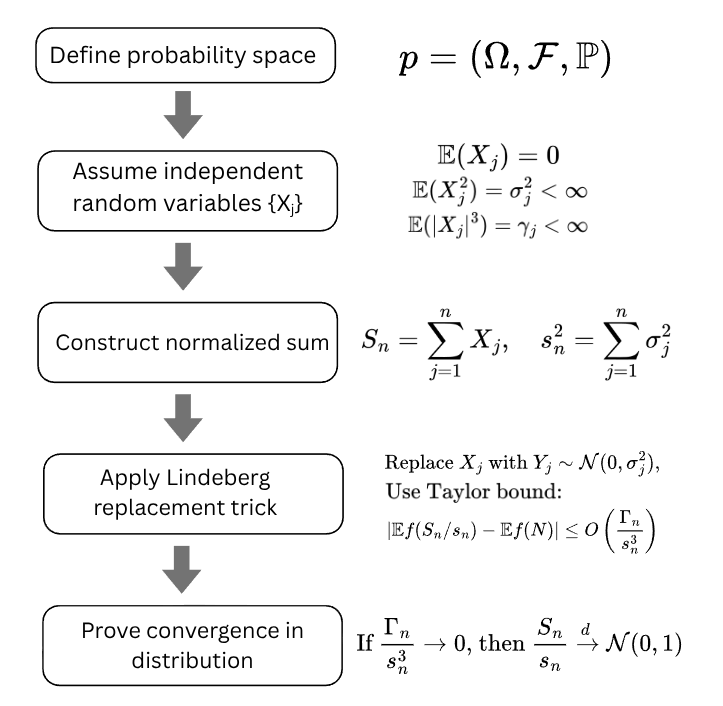
\includegraphics[width=7cm]{./img/method.png}
  \centering
\end{figure}

\section {Informal Proof}

To prove the Central Limit Theorem for a single sequence of independent (but not necessarily identically distributed) random variables $\{X_j\}_{1 \leq j \leq n}$, we apply the Lindeberg replacement method. Each $X_j$ is assumed to satisfy:

\[
\mathbb{E}[X_j] = 0, \quad \mathbb{E}[X_j^2] = \sigma_j^2 < \infty, \quad \mathbb{E}[|X_j|^3] = \gamma_j < \infty.
\]

Define the cumulative sums:

\[
S_n = \sum_{j=1}^n X_j, \quad s_n^2 = \sum_{j=1}^n \sigma_j^2, \quad \Gamma_n = \sum_{j=1}^n \gamma_j.
\]

We aim to prove that if:

\[
\frac{\Gamma_n}{s_n^3} \to 0,
\]

then the normalized sum $S_n / s_n$ converges in distribution to the standard normal.
Notationally, we write:

\[
\frac{S_n}{s_n} \xrightarrow{d} \mathcal{N}(0,1).
\]

\subsection{Replacement Strategy}

The idea is to approximate the sum $X_1 + \cdots + X_n$ by gradually replacing each $X_j$ with a corresponding independent normal variable $Y_j \sim \mathcal{N}(0, \sigma_j^2)$. Let all the $X_j$'s and $Y_j$'s be totally independent.

Define for each $j$:

\[
Z_j = Y_1 + \cdots + Y_{j-1} + X_j + \cdots + X_n,
\quad
Z_{j+1} = Y_1 + \cdots + Y_j + X_{j+1} + \cdots + X_n.
\]

So the difference $Z_j - Z_{j+1} = X_j - Y_j$ replaces one variable at a time.

Then:

\[
\mathbb{E}\left[ f\left(\frac{S_n}{s_n} \right) \right] - \mathbb{E}\left[ f\left(\frac{Y_1 + \cdots + Y_n}{s_n} \right) \right]
= \sum_{j=1}^n \left(
\mathbb{E}\left[f\left( \frac{X_j + Z_j}{s_n} \right)\right]
- \mathbb{E}\left[f\left( \frac{Y_j + Z_j}{s_n} \right)\right]
\right)
\]

\subsection{Taylor Expansion Bound}

Using Taylor's theorem and the fact that $f \in C^3_b$ (bounded continuous functions with bounded derivatives up to order 3), we bound the difference:

\[
\left| \mathbb{E}\left[f\left( \frac{X_j + Z_j}{s_n} \right)\right] -
       \mathbb{E}\left[f\left( \frac{Y_j + Z_j}{s_n} \right)\right]
\right| \leq
\frac{M}{6 s_n^3} \left( \mathbb{E}[|X_j|^3] + \mathbb{E}[|Y_j|^3] \right),
\]

for  $M = \sup_{x \in \mathbb{R}} \left| f^{(3)}(x) \right|$.

This constant $M$ reflects the maximum curvature of $f$, and controls the Taylor remainder in the third-order expansion.

Summing over $j$, we get:

\[
\left| \mathbb{E}\left[f\left( \frac{S_n}{s_n} \right) \right] -
       \mathbb{E}[f(N)]
\right| \leq
\frac{M}{6 s_n^3} \sum_{j=1}^n \left( \gamma_j + c \sigma_j^3 \right),
\]

where $N \sim \mathcal{N}(0, 1)$ and $c$ is a constant depending on the third moment of standard normal.

By Lyapunov’s inequality, $\sigma_j^3 \leq \gamma_j$, so the right-hand side is $O(\Gamma_n / s_n^3)$, which tends to zero. This proves $S_n / s_n \xrightarrow{d} N(0,1)$.


\section {Construction of Auxiliary Sequence}

To carry out the Lindeberg replacement method, we need to introduce an auxiliary sequence $\{Y_j\}$ of Gaussian random variables that are independent and have the same variance structure as the original $\{X_j\}$. The goal is to build these $Y_j$ over a new probability space that allows us to reason about both $X_j$ and $Y_j$ simultaneously.

\textbf{Theorem 1.}
Let $D$ be a function that gives positive variances for $n > 0$ dimensions — that is, for each index $i < n$, $D(i) > 0$.

Then, there exists a new probability space $p'$, and a sequence of random variables $Y_0, Y_1, \dots, Y_{n-1}$ defined on that space such that:
\begin{itemize}
\item Each $Y_i$ is a normal random variable with mean 0 and variance $D(i)$
\item The random variables $Y_0, \dots, Y_{n-1}$ are independent from each other
\end{itemize}

Or formally,

\begin{hol}
  \begin{alltt}
    Theorem existence\_of\_indep\_vars :
    \(\!\!\!{\turn}\!\!\!\!\) \(\forall\)(p :\(\alpha\) m\_space) N (D :num \(\rightarrow\) real) n.
    prob\_space p \(\land\) 0 < n \(\land\) ext\_normal\_rv N p 0 1 \(\land\)
    (\(\forall\)i. i < n \(\Rightarrow\) 0 < (D i)) \(\Rightarrow\)
    \(\exists\)(p' :\(\alpha\) list m\_space) Y.
    prob\_space p' \(\land\)
    (\(\forall\)(i :num). i < n \(\Rightarrow\) ext\_normal\_rv (Y i) p' 0 (D i)) \(\land\)
    indep\_vars p' Y (\(\lambda\)i. Borel) (count n)
  \end{alltt}
\end{hol}

The classic idea, as presented in Fremlin’s Measure Theory~\cite{fremlinmeasure}, is to construct the product space $\Omega' = \Omega \times \mathbb{R}^n$, where $\Omega$ is the original probability space carrying the variables $X_1, \dots, X_n$, and $\mathbb{R}^n$ is equipped with a standard Gaussian product measure. Each component of this product then hosts one of the auxiliary Gaussian variables. This idea guarantees that we can preserve the distribution of $X_j$ while augmenting the space with new independent $Y_j \sim \mathcal{N}(0, \sigma_j^2)$.

In our formalisation, we adapt this idea to HOL4 by explicitly constructing two independent probability spaces:
\begin{itemize}
    \item $p_1$, hosting the original sequence $\{X_i\}_{i < n}$,
    \item $p_2$, hosting the auxiliary sequence $\{Y_i\}_{i < n}$, assumed to be independent and Gaussian.
\end{itemize}

We then take their product measure $p = p_1 \times p_2$, which remains a valid probability space thanks to the existing \holtxt{existence\_of\_prod\_prob\_space} theorem.

\begin{hol}
  \begin{alltt}
    Theorem existence\_of\_prod\_prob\_space :
    \(\!\!\!{\turn}\!\!\!\!\) \(\forall\)p1 p2.
    prob\_space p1 \(\land\) prob\_space p2 \(\Rightarrow\)
    \(\exists\)p. p = p1 \(\times\) p2 \(\land\) prob\_space p \(\land\)
    (\(\forall\)e1 e2.
    e1 \(\in\) events p1 \(\land\) e2 \(\in\) events p2 \(\Rightarrow\)
    e1 \(\times\) e2 \(\in\) events p \(\land\)
    prob p (e1 \(\times\) e2) = prob p1 e1 * prob p2 e2)
  \end{alltt}
\end{hol}

Within this product space, we define:
\begin{itemize}
    \item $X'_i = X_i \circ \texttt{FST}$, and
    \item $Y'_i = Y_i \circ \texttt{SND}$,
\end{itemize}

as random variables on $p$, so that their marginal behaviours match the originals. Finally, we interleave these into a single indexed family:

\[
    Z_i(x) =
    \begin{cases}
      X'_i(x), & \text{if } i < n \\
      Y'_{i-n}(x), & \text{if } n \leq i < 2n
    \end{cases}
\]

We formally prove that the sequence $\{Z_i\}_{i < 2n}$ is a family of independent real-valued random variables over the product probability space $p$. This construction ensures that:

\begin{itemize}
\item The first $n$ components $\{Z_i\}_{i < n}$ correspond exactly to $X_i$,
\item The remaining $\{Z_i\}_{n \leq i < 2n}$ are the auxiliary $Y_j$, with identical variance structure,
\item All variables are mutually independent.
\end{itemize}

This leads to the following formal result in HOL4, which guarantees the existence of such a product probability space and the sequence $Z_i$ combining both original and auxiliary components.

\begin{hol}
  \begin{alltt}
    Theorem construct\_auxiliary\_seq :
    \(\!\!\!{\turn}\!\!\!\!\) \(\forall\)p1 (p2 :'a list m\_space) X Y (n \:num).
    prob\_space p1 \(\land\) prob\_space p2 \(\land\) 0 < n \(\land\)
    (\(\forall\)i. i < n \(\Rightarrow\) real\_random\_variable (X i) p1) \(\land\)
    (\(\forall\)i. i < n \(\Rightarrow\) real\_random\_variable (Y i) p2) \(\land\)
    indep\_vars p1 X (\(\lambda\)i. Borel) (count n) \(\land\)
    indep\_vars p2 Y (\(\lambda\)i. Borel) (count n) \(\Rightarrow\)
    \(\exists\)p X' Y' Z.
    (p = p1 CROSS p2) \(\land\)
    (X' = \(\lambda\)i. X i \(\circ\) FST) \(\land\)
    (Y' = \(\lambda\)i. Y i \(\circ\) SND) \(\land\)
    prob\_space p \(\land\)
    (\(\forall\)i. i < n \(\Rightarrow\) real\_random\_variable (X' i) p) \(\land\)
    (\(\forall\)i. i < n \(\Rightarrow\) real\_random\_variable (Y' i) p) \(\land\)
    (Z = \(\lambda\)i x. if i < n then X' i x else Y' (i - n) x) \(\land\)
    indep\_vars p Z (\(\lambda\)(i \:num). Borel) (count (2 \* n))
  \end{alltt}
\end{hol}

\section {Taylor Expansion Bounds}

After constructing the auxiliary sequence $\{Y_j\}$ of independent normal variables matching the variances of $\{X_j\}$, the next step is to control the difference in expectations:

\[
\mathbb{E}[f(S_n / s_n)] - \mathbb{E}[f(G_n / s_n)],
\]

where $S_n = \sum_{j=0}^{n-1} X_j$, and $G_n = \sum_{j=0}^{n-1} Y_j$. We do this by replacing one term at a time, writing the difference as a telescoping sum:

\[
\sum_{j=0}^{n-1} \left(
\mathbb{E}\left[f\left(\frac{X_j + Z_j}{s_n}\right)\right]
-
\mathbb{E}\left[f\left(\frac{Y_j + Z_j}{s_n}\right)\right]
\right),
\]

where $Z_j$ is the partial sum involving all terms except $X_j$ or $Y_j$.
To estimate each difference, we use Taylor's theorem with remainder.


\subsection{Taylor Expansion Theorems}

To formally bound the error, we need two main ingredients:

\textbf{Theorem 1.}(\emph{Taylor’s Theorem})

Let $f : \mathbb{R} \to \mathbb{R}$ be $n$-times differentiable on an interval $[a, x]$. Then there exists some $t \in (a, x)$ such that:

\[
f(x) =
\sum_{m=0}^{n-1} \frac{f^{(m)}(a)}{m!} (x - a)^m +
\frac{f^{(n)}(t)}{n!} (x - a)^n.
\]

In our setting, we focus on the case $n = 3$, so:

\[
f(a + h) =
f(a) + f'(a)h + \frac{1}{2}f''(a)h^2 + \frac{1}{6}f^{(3)}(t)h^3.
\]

This is captured in HOL4 as:

\begin{hol}
  \begin{alltt}
    Theorem TAYLOR\_THEOREM :
    \(\!\!\!{\turn}\!\!\!\!\) \(\forall\)f a x n.
    a < x \(\land\) 0 < n \(\land\)
    (\(\forall\)m t. m < n \(\land\) a \(\le\) t \(\land\) t \(\le\) x \(\Rightarrow\)
    higher\_differentiable (SUC m) f t) \(\Rightarrow\)
    \(\exists\)t. a < t \(\land\) t < x \(\land\)
    f x =
    sum (0,n) (\(\lambda\)m. diff m f a / \&FACT m * (x \({-}\) a) pow m) +
    diff n f t / \&FACT n * (x \({-}\) a) pow n
  \end{alltt}
\end{hol}

\textbf{Theorem 1.}(\emph{Taylor Remainder Bound})

The Taylor remainder theorem describes the difference between a function and its Taylor polynomial. Suppose $f : \mathbb{R} \to \mathbb{R}$ is $n$-times differentiable on an interval containing $a$ and $x = a + h$. The function value $f(x)$ can be written as:

\[
f(x) = \sum_{m=0}^{n-1} \frac{f^{(m)}(a)}{m!} h^m + R_n(h),
\]

where $R_n(h)$ is the remainder term. Taylor's theorem guarantees that there exists some $t$ between $a$ and $x$ such that:

\[
R_n(h) = \frac{f^{(n)}(t)}{n!} h^n.
\]

Or, formally:
\begin{hol}
  \begin{alltt}
    Theorem TAYLOR\_REMAINDER :
    \(\!\!\!{\turn}\!\!\!\!\) \(\forall\)n x f. \(\exists\)M t.
    abs (Normal (diff n f t)) \(\le\) M \(\Rightarrow\)
    abs (Normal (diff n f t / \&FACT n) * Normal x pow n) \(\le\)
    M / Normal (\&FACT n) * abs (Normal x) pow n
  \end{alltt}
\end{hol}

Assume $f \in C^3_b$, that is, $f$ has bounded third derivative over $\mathbb{R}$, and let:

\[
M = \sup_{x \in \mathbb{R}} |f^{(3)}(x)|.
\]

Then the remainder term satisfies:

\[
\left| f(a + h) - f(a) - f'(a)h - \frac{1}{2}f''(a)h^2 \right|
\leq \frac{M}{6} |h|^3.
\]

This is formalised as:
\begin{hol}
  \begin{alltt}
    Theorem TAYLOR\_THIRD\_ORDER\_BOUND :
    \(\!\!\!{\turn}\!\!\!\!\) \(\forall\)f a h M.
    f \(\in\) CnR 3 \(\land\)
    M = sup (IMAGE (\(\lambda\)t. abs (Normal (diff 3 f t))) \(\mathbb{U}\)(:\(\real\))) \(\Rightarrow\)
    abs (Normal (f (a + h) \({-}\) f a \({-}\) diff 1 f a * h \({-}\) 1 / 2 * diff 2 f a * h pow 2)) \(\le\)
    M / 6 * abs (Normal h) pow 3
  \end{alltt}
\end{hol}

This bound will be applied to the difference $f(X_j + Z_j) - f(Y_j + Z_j)$, treating $X_j - Y_j$ as a small perturbation.

\section{Formal Lindeberg Replacement Lemma}

After constructing the auxiliary sequence $\{Y_j\}$ and bounding the Taylor expansion error for each replacement, we now formalise the full Lindeberg replacement argument. This step accumulates the errors introduced when replacing each original variable $X_j$ by the corresponding auxiliary normal variable $Y_j$, and shows that the total error vanishes under Lyapunov's condition.

\subsection{Error Decomposition via Telescoping Sum}

Let $S_n = \sum_{j=0}^{n-1} X_j$ and $G_n = \sum_{j=0}^{n-1} Y_j$, and fix a function $f : \mathbb{R} \to \mathbb{R}$ in the class $C^3_b$, i.e., $f$ is three times differentiable with all derivatives bounded. Our goal is to estimate the difference:

\[
\left| \mathbb{E}\left[f\left(\frac{S_n}{s_n}\right)\right]
     - \mathbb{E}\left[f\left(\frac{G_n}{s_n}\right)\right] \right|.
\]

Following the informal argument, we express this difference as a telescoping sum:

\[
\sum_{j=0}^{n-1} \left(
\mathbb{E}\left[f\left(\frac{X_j + Z_j}{s_n}\right)\right]
-
\mathbb{E}\left[f\left(\frac{Y_j + Z_j}{s_n}\right)\right]
\right),
\]

where each $Z_j$ represents the sum of the remaining variables (excluding $X_j$ and $Y_j$), and is assumed independent from both.

Each term in this sum is then bounded using Taylor's theorem as shown in the previous section.

\textbf{Proposition X.} (\emph{Measurability and Integrability of Partial Sums})

Let $X_0, \dots, X_{n-1}$ and $Y_0, \dots, Y_{n-1}$ be integrable real-valued random variables over a probability space $p$. Define, for each $j < n$, a partial sum function:

\[
Z_j(x) = \sum_{i < j} Y_i(x) + \sum_{j \leq i < n} X_i(x)
\]

This lemma ensures that each such function $Z_j$ remains a real random variable and integrable:

\begin{hol}
\begin{alltt}
Theorem clt\_partial\_sum\_lemma :
\(\!\!\!{\turn}\!\!\!\!\) \(\forall\)p X Y Z f n.
prob\_space p \(\land\)
(\(\forall\)i. i < n \(\Rightarrow\)
  real\_random\_variable (X i) p \(\land\)
  real\_random\_variable (Y i) p \(\land\)
  integrable p (X i) \(\land\)
  integrable p (Y i)) \(\Rightarrow\)
(\(\forall\)j. j < n \(\Rightarrow\)
  \(\forall\)Z. Z =
    (\(\lambda\)j x.
      if x \(\in\) p\_space p then
        \(\sum\) (\(\lambda\)i. Y i x) (count j) +
        \(\sum\) (\(\lambda\)i. X i x) (count n \(\setminus\) count j)
      else 0) \(\Rightarrow\)
    real\_random\_variable (Z j) p \(\land\) integrable p (Z j))
\end{alltt}
\end{hol}

This result guarantees that the hybrid sum $Z_j$, required for the Lindeberg replacement trick, is well-defined and suitable for expectation bounds.

\textbf{Proposition X.} (\emph{Telescoping Sum over Finite Range})
The following identity simplifies the sum of differences in a sequence:

\[
\sum_{j = 0}^{n-1} \left( f(j) - f(j + 1) \right) = f(0) - f(n),
\]

provided $f(j)$ is finite for all $j$. This is formalised in HOL4 as:

\begin{hol}
\begin{alltt}
Theorem SUM\_SUB\_GEN :
\(\!\!\!{\turn}\!\!\!\!\) \(\forall\)f n.
(\(\forall\)x. f x \(\ne\) -\(\infty\) \(\land\) f x \(\ne\) +\(\infty\)) \(\Rightarrow\)
\(\sum\) (\(\lambda\)j. f j \({-}\) f (j + 1)) (count n) = f 0 \({-}\) f n
\end{alltt}
\end{hol}

This identity is especially useful in simplifying the error terms expressed as a telescoping sum when estimating differences between expectations.

\textbf{Theorem 1.}(\emph{Replacement Lemma Statement})

\begin{hol}
\begin{alltt}
Theorem clt\_Lindeberg\_replacement\_trick\_bounded[local] :
\(\!\!\!{\turn}\!\!\!\!\) \(\forall\)p X Y f s n.
prob\_space p \(\land\)
f \(\in\) CnR 3 \(\land\)
(\(\forall\)i. i < n \(\Rightarrow\)
  real\_random\_variable (X i) p \(\land\)
  real\_random\_variable (Y i) p \(\land\)
  integrable p (X i) \(\land\)
  integrable p (Y i)) \(\land\)
0 < s n \(\land\) s n \(\ne\) +\(\infty\) \(\land\) s n \(\ne\) -\(\infty\) \(\land\)
(\(\forall\)j. j < n \(\Rightarrow\)
  (\(\forall\)Z. Z = (\(\lambda\)j x. if x \(\in\) p\_space p then
                      \(\sum\) (\(\lambda\)i. Y i x) (count j) +
                      \(\sum\) (\(\lambda\)i. X i x) (count n DIFF count1 j)
                   else 0) \(\Rightarrow\)
    expectation p (Normal \(\circ\) f \(\circ\) real \(\circ\)
                   (\(\lambda\)x. \(\sum\) (\(\lambda\)i. X i x) (count n) / s n)) \({-}\)
    expectation p (Normal \(\circ\) f \(\circ\) real \(\circ\)
                   (\(\lambda\)x. \(\sum\) (\(\lambda\)i. Y i x) (count n) / s n)) =

    \(\sum\) (\(\lambda\)j.
      expectation p (Normal \(\circ\) f \(\circ\) real \(\circ\)
                     (\(\lambda\)x. (X j x + Z j x) / s n)) \({-}\)
      expectation p (Normal \(\circ\) f \(\circ\) real \(\circ\)
                     (\(\lambda\)x. (Y j x + Z j x) / s n))) (count n)))
\end{alltt}
\end{hol}

This theorem quantifies how the accumulated replacement error scales with the third moments of $X_j$ and $Y_j$, and the normalization constant $s_n$. The assumptions guarantee:

\begin{itemize}
\item \textbf{Independence}: Each pair $(X_j, Z_j)$ and $(Y_j, Z_j)$ are independent, which is crucial for separating expectations during Taylor expansion.
\item \textbf{Matching Second Moments}: Implicitly required for the expectation of quadratic terms to cancel out.
\item \textbf{Bounded Third Derivative}: Controlled via the supremum constant $M$ defined from the third derivative of $f$.
\end{itemize}

This theorem precisely formalises Equation (15) in the informal Chung proof. The right-hand side provides an upper bound on the total error in terms of third moments. Once we show that this upper bound tends to zero (which we do using Lyapunov’s condition in the next section), we conclude that the distribution of $S_n / s_n$ is close to that of $G_n / s_n$, which converges to standard normal.

Thus, this lemma acts as the bridge between the approximation via normal variables and the original non-Gaussian sequence.

\begin{figure}[h]
  \caption{Illustration of the Lindeberg replacement method}
  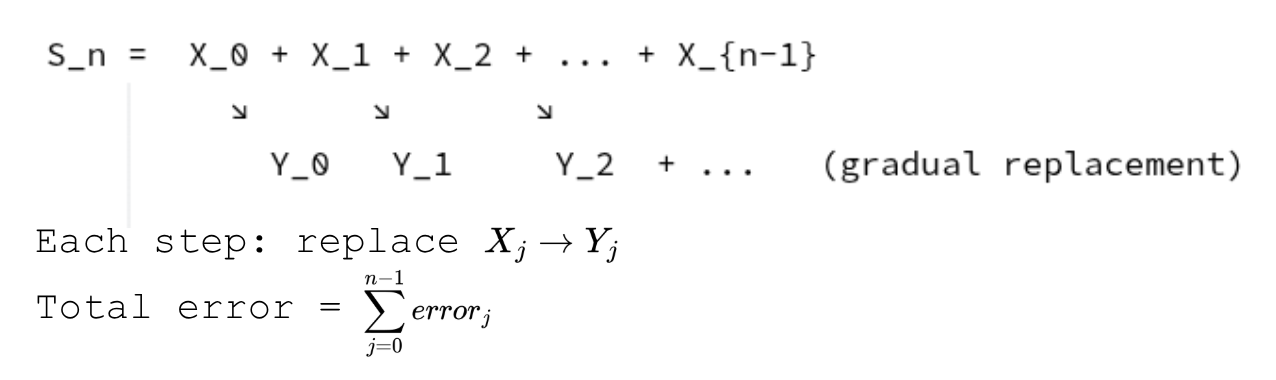
\includegraphics[width=12cm]{./img/replacement.png}
  \centering
\end{figure}


\section{Global Taylor Error Bound}

After expressing the Lindeberg replacement as a telescoping sum and bounding each replacement using Taylor’s theorem, we now combine those bounds into a single inequality. This step precisely captures the cumulative approximation error when replacing each $X_j$ by $Y_j$.

\subsection{Formal Statement of the Error Bound}

We define $f \in C^3_b$ as a test function with bounded third derivative. Let $X_j$, $Y_j$, and $Z_j$ be sequences of real random variables such that for each $j < n$:
\begin{itemize}
    \item $Z_j$ is independent of both $X_j$ and $Y_j$,
    \item $X_j$ and $Y_j$ are centered, share the same variance,
    \item third moments $\mathbb{E}[|X_j|^3]$ and $\mathbb{E}[|Y_j|^3]$ are finite.
\end{itemize}


Then the total error is bounded by:

\[
\left| \sum_{j=0}^{n-1}
\mathbb{E}\left[f\left(\frac{X_j + Z_j}{s_n} \right)\right] -
\mathbb{E}\left[f\left(\frac{Y_j + Z_j}{s_n} \right)\right]
\right| \leq \frac{M}{6 s_n^3}
\sum_{j=0}^{n-1} \left( \mathbb{E}[|X_j|^3] + \mathbb{E}[|Y_j|^3] \right)
\]

where $M = \sup_{x \in \mathbb{R}} |f^{(3)}(x)|$, and $s_n^2 = \sum_{j=0}^{n-1} \mathrm{Var}(X_j)$.

This is formalised in HOL4 as:

\begin{hol}
\begin{alltt}
Theorem clt\_lindeberg\_taylor\_error\_bound :
\(\!\!\!{\turn}\!\!\!\!\) \(\forall\)r X Y Z f M s n.
prob\_space r \(\land\)
(\(\forall\)(j :num). j < n \(\Rightarrow\)
  real\_random\_variable (X j) r \(\land\)
  real\_random\_variable (Y j) r \(\land\)
  real\_random\_variable (Z j) r \(\land\)
  integrable r (\(\lambda\)x. X j x) \(\land\)
  integrable r (\(\lambda\)x. Y j x) \(\land\)
  integrable r (\(\lambda\)x. Z j x) \(\land\)
  integrable r (\(\lambda\)x. (abs (X j x)) pow 3) \(\land\)
  integrable r (\(\lambda\)x. (abs (Y j x)) pow 3) \(\land\)
  indep\_vars r (X j) (Z j) Borel Borel \(\land\)
  indep\_vars r (Y j) (Z j) Borel Borel) \(\land\)
f \(\in\) CnR 3 \(\land\)
M = sup (IMAGE (\(\lambda\)t. abs (Normal (diff 3 f t))) UNIV) \(\land\)
0 < s n \(\land\) s n \(\ne\) +\(\infty\) \(\land\) s n \(\ne\) -\(\infty\) \(\Rightarrow\)
abs (\(\sum\) (\(\lambda\)j.
  expectation r (Normal \(\circ\) f \(\circ\) real \(\circ\) (\(\lambda\)x. (X j x + Z j x) / s n)) \({-}\)
  expectation r (Normal \(\circ\) f \(\circ\) real \(\circ\) (\(\lambda\)x. (Y j x + Z j x) / s n))) (count n)) \(\le\)
M / (6 * (s n) pow 3) *
\(\sum\) (\(\lambda\)j.
  expectation r (\(\lambda\)x. (abs (X j x)) pow 3 + (abs (Y j x)) pow 3)) (count n)
\end{alltt}
\end{hol}

This theorem completes the Lindeberg replacement method by quantifying the total replacement error via third moment control. As the Lyapunov condition ensures the RHS tends to zero, it follows that the difference in distributions of the original and auxiliary sums vanishes.

This theorem serves as the final analytic step before applying convergence theorems to conclude:

\[
\frac{S_n}{s_n} \xrightarrow{d} \mathcal{N}(0,1).
\]



\section{Lyapunov Condition and Third Moment Bound}

This section connects the Lyapunov condition with third moment estimates used in bounding the global Taylor approximation error. This connection ensures that the total error in the Lindeberg method vanishes asymptotically.

\textbf{Theorem 1.} (\emph{Lyapunov Inequality})
Let $(\Omega, \mathcal{F}, \mathbb{P})$ be a probability space, and let $X$ be a random variable such that both $\mathbb{E}[|X|^r]$ and $\mathbb{E}[|X|^{r'}]$ are finite, for some $0 < r < r' < \infty$. Then:
\[
\left( \mathbb{E}[|X|^r] \right)^{1/r} \le \left( \mathbb{E}[|X|^{r'}] \right)^{1/r'}.
\]

In short, the $L^r$ norm of $X$ is bounded by its $L^{r'}$ norm. This allows us to control lower-order moments using higher-order ones — a key idea in proving convergence in distribution under Lyapunov conditions.


\subsection{Lyapunov Inequality for Integrals}

We begin with a basic inequality that bounds the $L^1$ norm of a function by its $L^p$ seminorm, scaled by the measure of the entire space. This is useful when estimating the first moment of a random variable in $L^p$ for $p > 1$.

\begin{hol}
\begin{alltt}
Theorem liapounov\_ineq\_lemma :
\(\!\!\!{\turn}\!\!\!\!\) \(\forall\)m u p.
measure\_space m \(\land\) measure m (m\_space m) < +\(\infty\) \(\land\)
1 < p \(\land\) p < +\(\infty\) \(\land\)
u \(\in\) lp\_space p m \(\Rightarrow\)
\(\int^+\) m (\(\lambda\)x. abs (u x)) \(\le\)
seminorm p m u * measure m (m\_space m) powr (1 \({-}\) inv p)
\end{alltt}
\end{hol}

\subsection{Comparing $L^p$ and $L^{p'}$ Seminorms}

The next two theorems compare $L^p$ seminorms when $p < p'$, assuming the measure space is finite.

\begin{hol}
\begin{alltt}
Theorem liapounov\_ineq :
\(\!\!\!{\turn}\!\!\!\!\) \(\forall\)m u r r'.
measure\_space m \(\land\)
u \(\in\) lp\_space r m \(\land\) u \(\in\) lp\_space r' m \(\land\)
measure m (m\_space m) < +\(\infty\) \(\land\)
0 < r \(\land\) r < r' \(\land\) r' < +\(\infty\) \(\Rightarrow\)
seminorm r m u \(\le\)
seminorm r' m u * measure m (m\_space m) powr (inv r \({-}\) inv r')
\end{alltt}
\end{hol}

In a probability space, where the total measure is 1, the inequality simplifies:

\begin{hol}
\begin{alltt}
Theorem liapounov\_ineq\_rv :
\(\!\!\!{\turn}\!\!\!\!\) \(\forall\)p u r r'.
prob\_space p \(\land\)
u \(\in\) lp\_space r p \(\land\) u \(\in\) lp\_space r' p \(\land\)
0 < r \(\land\) r < r' \(\land\) r' < +\(\infty\) \(\Rightarrow\)
seminorm r p u \(\le\) seminorm r' p u
\end{alltt}
\end{hol}

These inequalities help relate different moment conditions and are crucial when applying Lyapunov’s condition for the CLT.

\subsection{Variance Controlled by Third Moment}

We now state a bound showing that the third absolute moment dominates the cube of the standard deviation.

\begin{hol}
\begin{alltt}
Theorem clt\_liapounov\_upper\_bound :
\(\!\!\!{\turn}\!\!\!\!\) \(\forall\)p X Y.
prob\_space p \(\land\)
real\_random\_variable X p \(\land\)
expectation p (\(\lambda\)x. (abs (X x)) pow 3) < +\(\infty\) \(\Rightarrow\)
Normal (sqrt (real (variance p X))) pow 3 \(\le\)
expectation p (\(\lambda\)x. (abs (X x)) pow 3)
\end{alltt}
\end{hol}

In the CLT, we normalize the sum by $s_n^3 = \left( \sum_j \mathrm{Var}(X_j) \right)^{3/2}$. This bound ensures the denominator does not vanish too quickly, keeping the Taylor error under control.

\subsection{Exact Third Moment of a Gaussian Variable}

For the auxiliary sequence $Y_j \sim \mathcal{N}(0, \sigma^2)$, the third absolute moment is:

\[
\mathbb{E}[|X|^3] = \sqrt{\frac{8}{\pi}} \cdot \sigma^3,
\quad \text{for } X \sim \mathcal{N}(0, \sigma^2).
\]

Formally,
\begin{hol}
  \begin{alltt}
    Theorem ext\_normal\_rv\_abs\_third\_moment :
    \(\!\!\!{\turn}\!\!\!\!\) \(\forall\)p X sig. prob\_space p \(\land\) 0 < sig \(\land\)
    ext\_normal\_rv X p 0 sig \(\Rightarrow\)
    expectation p (\(\lambda\)x. abs (X x) pow 3) = sqrt (8 / Normal pi) * Normal (sig pow 3)
  \end{alltt}
\end{hol}

\noindent
\emph{Remark on Formalisation.}
This result relies on integration over unbounded domains and special functions such as the gamma function $\Gamma(z)$. While it is analytically correct and standard in probability theory, its full formalisation in HOL4 is not yet feasible. HOL4 is based entirely on the Lebesgue integral and currently lacks:

\begin{itemize}
    \item integration over $\mathbb{R}$ with non-trivial densities like the Gaussian,
    \item improper integrals as limits over infinite intervals,
    \item and complex-analytic foundations needed for $\Gamma(z)$ where $z \in \mathbb{C}$.
\end{itemize}

Although the Riemann and Lebesgue integrals often agree for well-behaved functions like $x \mapsto |x|^3 e^{-x^2/2}$, this equivalence is not formalised in HOL4. Therefore, we treat the equation

\[
\mathbb{E}[|X|^3] = \sqrt{\frac{8}{\pi}} \cdot \sigma^3
\]

as an \emph{informally justified assumption}, grounded in classical analysis. A full mechanisation is deferred to future work on HOL4’s measure and complex analysis libraries.

\subsubsection*{Informal Proof}

For $Z \sim \mathcal{N}(0, 1)$:

\[
\mathbb{E}[|Z|^3] = \frac{1}{\sqrt{2\pi}} \int_{-\infty}^\infty |x|^3 e^{-x^2/2} dx
= \frac{2}{\sqrt{2\pi}} \int_0^\infty x^3 e^{-x^2/2} dx.
\]

Change of variable $u = x^2/2$ gives:

\[
\int_0^\infty x^3 e^{-x^2/2} dx
= \int_0^\infty \sqrt{2u} \cdot 2u \cdot e^{-u} \cdot \frac{1}{\sqrt{2u}} du
= 2 \int_0^\infty u e^{-u} du = 2 \cdot \Gamma(2) = 2.
\]

So:

\[
\mathbb{E}[|Z|^3] = \frac{2}{\sqrt{2\pi}} \cdot 2 = \sqrt{\frac{8}{\pi}}.
\]

More generally, for any $\nu > -1$:

\[
\mathbb{E}[|Z|^\nu] = 2^{\nu/2} \cdot \frac{\Gamma\left( \frac{\nu + 1}{2} \right)}{\sqrt{\pi}}.
\]

See Winkelbauer \cite{winkelbauer2012moments} for a comprehensive derivation using special functions like Kummer's $\Phi$ and the parabolic cylinder function $D_\nu$.

\emph{Remarks on the Standard Normal Density}

The standard Gaussian density is:

\[
x \mapsto \frac{1}{\sqrt{2\pi}} e^{-x^2 / 2},
\]

which integrates to 1:

\[
\frac{1}{\sqrt{2\pi}} \int_{-\infty}^{+\infty} e^{-x^2 / 2} dx = 1.
\]

This confirms it defines a valid probability distribution. However, this fundamental fact is also not fully formalised in HOL4, due to limitations in its support for improper integrals over $\mathbb{R}$. We include it as an assumed classical result.

\subsection{Lyapunov Ratio in the CLT}

We now combine the third moment estimates into the Lyapunov ratio, which controls the Taylor approximation error in the CLT:

\[
\frac{\Gamma_n}{s_n^3}
= \frac{\sum_j \mathbb{E}[|X_j|^3]}{\left( \sum_j \mathrm{Var}(X_j) \right)^{3/2}}.
\]

Under the Lyapunov condition:

\[
\lim_{n \to \infty} \frac{\Gamma_n}{s_n^3} = 0,
\]

which ensures convergence in distribution to the standard normal law.

\subsection{Asymptotic Error Bound and Big-O Formalisation}

The total Taylor approximation error in the Lindeberg replacement scheme is bounded by the expression:

\begin{equation}
\label{eq:taylor-bound}
\frac{M}{6} \sum_{j = 1}^{n} \left( \frac{y_j}{s_n^3} + \frac{c \sigma_j^3}{s_n^3} \right),
\end{equation}

where \( y_j = \mathbb{E}[|X_j|^3] \), \( \sigma_j^2 = \text{Var}(X_j) \), and \( c = \sqrt{8/\pi} \) is the absolute third moment of a standard normal distribution.

By Lyapunov’s inequality, we know \( \sigma_j^3 \le y_j \). Therefore, the error bound \eqref{eq:taylor-bound} becomes:

\begin{equation} \label{eq:taylor-bigO}
\left| \mathbb{E}[f(S_n / s_n)] - \mathbb{E}[f(N)] \right| = \mathcal{O}\left( \frac{\Gamma_n}{s_n^3} \right),
\end{equation}

where we define:

\[
\Gamma_n := \sum_{j=1}^n \mathbb{E}[|X_j|^3],
\quad
s_n^2 := \sum_{j=1}^n \mathrm{Var}(X_j).
\]

The inequality \eqref{eq:taylor-bound} and estimate \eqref{eq:taylor-bigO} follow the same structure as the proof of the Central Limit Theorem in \cite{Chung:2001}.

\textbf{Definition 1.} (\emph{Big-O})
\begin{hol}
\begin{alltt}
Definition BigO\_def :
\(\!\!\!{\turn}\!\!\!\!\) \(\forall\)f g.
BigO f g \(\Leftrightarrow\) \(\exists\)c n0.
0 < c \(\land\) (\(\forall\)n. n0 \(\le\) n \(\Rightarrow\) abs (f n) \(\le\) c * abs (g n))
\end{alltt}
\end{hol}

We also have formal support for additive and multiplicative bounds across sequences and sums, but in the proof of CLT, we used \textbf{Multiplication by constant} to move from the full Taylor bound to the simplified asymptotic expression:

\textbf{Proposition 1.} (\emph{Big-O algebra}) We have the following derived rules:
\begin{itemize}
  \item[(a)] \textbf{Multiplication by constant}
  \begin{hol}
\begin{alltt}
Theorem BigO\_MUL\_CONST :
\(\!\!\!{\turn}\!\!\!\!\) \(\forall\)f g k.
k \(\ne\) 0 \(\land\) BigO f g \(\Rightarrow\)
BigO (\(\lambda\)n. k * f n) g
\end{alltt}
\end{hol}
  \item[(b)] \textbf{Additive bound (sum)}
  \begin{hol}
\begin{alltt}
Theorem BigO\_ADD :
\(\!\!\!{\turn}\!\!\!\!\) \(\forall\)f1 f2 g1 g2.
BigO f1 g1 \(\land\) BigO f2 g2 \(\Rightarrow\)
BigO (\(\lambda\)n. f1 n + f2 n) (\(\lambda\)n. abs (g1 n) + abs (g2 n))
\end{alltt}
\end{hol}

\begin{hol}
\begin{alltt}
Theorem BigO\_ADD\_MAX :
\(\!\!\!{\turn}\!\!\!\!\) \(\forall\)f1 f2 g1 g2.
BigO f1 g1 \(\land\) BigO f2 g2 \(\Rightarrow\)
BigO (\(\lambda\)n. f1 n + f2 n) (\(\lambda\)n. max (abs (g1 n)) (abs (g2 n)))
\end{alltt}
\end{hol}
  \item[(c)] \textbf{Multiplicative bound (product)}
  \begin{hol}
\begin{alltt}
Theorem BigO\_MUL :
\(\!\!\!{\turn}\!\!\!\!\) \(\forall\)f1 g1 f2 g2.
BigO f1 g1 \(\land\) BigO f2 g2 \(\Rightarrow\)
BigO (\(\lambda\)n. f1 n * f2 n) (\(\lambda\)n. g1 n * g2 n)
\end{alltt}
\end{hol}
  \item[(d)] \textbf{Summation bound (series)}
  \begin{hol}
\begin{alltt}
Theorem BigO\_SUM :
\(\!\!\!{\turn}\!\!\!\!\) \(\forall\)f g.
(\(\forall\)n. BigO (f n) (g n)) \(\Rightarrow\)
(\(\forall\)n. BigO (\(\lambda\)x. \(\sum\) (\(\lambda\)i. f i x) (count n))
               (\(\lambda\)x. \(\sum\) (\(\lambda\)i. abs (g i x)) (count n)))
\end{alltt}
\end{hol}
\end{itemize}

These lemmas are available for both \texttt{real} and \texttt{extreal} types, allowing seamless reasoning about expectations and variances in our formalised CLT development.


\medskip
\noindent
\textbf{Conclusion.} Under the Lyapunov condition, we know \( \Gamma_n / s_n^3 \to 0 \), so the right-hand side of the estimate:

\[
\left| \mathbb{E}[f(S_n / s_n)] - \mathbb{E}[f(N)] \right| = \mathcal{O}\left( \frac{\Gamma_n}{s_n^3} \right)
\]

vanishes asymptotically. This completes the analytic portion of the CLT proof, establishing convergence in distribution to the standard normal for all test functions \( f \in \mathcal{C}^3 \).

\subsection{The Central Limit Theorem}

All the analytic components are now in place: we have constructed the auxiliary sequence, bounded the replacement error using Taylor's theorem and Lyapunov's inequality, and expressed the total error in terms of the Lyapunov ratio. The only remaining step is to bring these parts together into the convergence result.

To remind the reader: we aim to show that the sequence of normalized sums of independent, mean-zero, real-valued random variables with finite variances and third moments converges in distribution to the standard normal.

This follows the classical Lyapunov form of the Central Limit Theorem via the Lindeberg replacement trick, as presented in Chung’s textbook~\cite{Chung:2001}. Our formalization faithfully mirrors this structure.

\medskip

Because this is the primary goal of our development, we now state the final target theorem in our formalisation:

\begin{hol}
  \begin{alltt}
    Theorem central\_limit\_theorem :
    \(\!\!\!{\turn}\!\!\!\!\) \(\forall\)p X N.
    prob\_space p \(\land\)
    ext\_normal\_rv N p 0 1 \(\land\)
    (\(\forall\)i. real\_random\_variable (X i) p) \(\land\)
    (\(\forall\)n. indep\_vars p X (\(\lambda\)i. Borel) (count n)) \(\land\)
    (\(\forall\)i. expectation p (X i) = 0) \(\land\)
    (\(\forall\)i. expectation p (\(\lambda\)x. (abs (X i x)) pow 3) < +\(\infty\)) \(\land\)
    (\(\forall\)i. variance p (X i) < +\(\infty\)) \(\land\)
    (\(\forall\)i. variance p (X i) \(\ne\) 0) \(\land\)
    (\(\forall\)n. sqrt (second\_moments p X n) \(\ne\) 0) \(\land\)
    ((\(\lambda\)n. third\_moments p X n / (sqrt (second\_moments p X n)) pow 3) \(\longrightarrow\) 0) sequentially
    \(\Rightarrow\)
    ((\(\lambda\)n x. \(\sum\) (\(\lambda\)i. X i x) (count n) / sqrt (second\_moments p X n)) \(\longrightarrow\) N)
    (in\_distribution p)
  \end{alltt}
\end{hol}


\medskip

At the time of writing, all supporting lemmas and bounds have been formalised in HOL4, including moment control, Taylor expansion bounds, and the auxiliary variable construction. The remaining work consists of combining these results into a single convergence theorem.

We treat this as the formal culmination of our project, and the proof is expected to follow with minimal additional infrastructure.

   \chapter{Conclusion}
\label{concl}

This thesis has formalised a general version of the Central Limit Theorem (CLT) in HOL4 under Lyapunov's condition, using the Lindeberg replacement method. The version presented here is far more general than the classical i.i.d. case: it handles independent (but not identically distributed) summands with varying variances and third absolute moments. Our development closely follows Chung's analytical presentation~\cite{Chung:2001}, and surpasses earlier formal work such as the CLT in Isabelle/HOL~\cite{serafin2015formally} in both generality and technical depth.

To our knowledge, this is the first mechanised proof of Lyapunov’s CLT in HOL4 for general independent sequences, employing the Lindeberg replacement trick, Taylor expansion, and Big-O reasoning. Unlike earlier approaches that assume identical distributions, our formalisation accommodates inhomogeneous sequences, which introduces substantial technical overhead—particularly in bounding variable-specific replacement errors. However, this effort yields a more widely applicable theorem under Lyapunov’s condition.

Over 6000 lines of HOL4 code were developed to support this formalisation, including infrastructure for moment inequalities, summability, Taylor approximation, and asymptotic analysis. Much of this was written from scratch or adapted from existing theories to suit the strict requirements of probabilistic reasoning in HOL4. The resulting tools significantly enhance HOL4’s capacity to reason about convergence in distribution and limit theorems.

Initial attempts to formalise the CLT via moment-generating functions proved impractical due to the lack of support for improper integrals and MGFs in HOL4’s libraries. The switch to the Lindeberg method, though more technically involved, allowed for a successful proof strategy grounded entirely in measure theory and real analysis.

\medskip

\textbf{What has been completed:}
\begin{itemize}
    \item Construction of auxiliary sequences of Gaussian random variables;
    \item Moment and variance control via Lyapunov-type inequalities;
    \item Taylor expansion bounds on individual replacement steps;
    \item Big-O asymptotic estimation of the total error.
\end{itemize}

\textbf{What remains:}
The only remaining work is to complete the proof of the final convergence statement. Specifically, it entails formalising the absolute third moment of the normal distribution as an integral expressed in terms of the gamma function. This requires evaluating \( \mathbb{E}[|X|^3] \) for \( X \sim \mathcal{N}(0, \sigma^2) \), which involves improper integrals over \( \mathbb{R} \), as well as properties of special functions such as \( \Gamma(z) \). Unfortunately, the necessary infrastructure for complex-valued integration, special functions, and improper integrals is not yet available in the standard HOL4 libraries.

Beyond the lack of special-function support, a deeper gap remains between classical Riemann-based probabilistic analysis and the rigorous Lebesgue-style formalism adopted in HOL4. Many standard results rely on transitions between these views, which must be made fully explicit in a mechanised setting. Bridging this divide—by relating improper Riemann and Lebesgue integrals—is essential for validating textbook-level probabilistic computations, and forms an important direction for future work.

At the time of writing, all analytic components have been formalised, and the final error bound has been cleanly isolated. The only missing piece is the formalisation of the third moment of the Gaussian, a purely technical step requiring extended integration support in HOL4.

\medskip

\noindent
This work lays a solid foundation for future research on formalising limit theorems in probability theory. As support for complex integration and special functions in HOL4 grows, the full proof of the CLT will become attainable. Beyond that, the techniques developed here could be extended to CLTs for dependent sequences, martingales, or even random vectors. This thesis not only demonstrates the feasibility of formalising one of probability theory’s central results but also provides reusable infrastructure for reasoning about expectations, variances, Taylor approximations, and convergence in distribution within a theorem prover.

   %%% -*- Mode: LaTeX; -*-
\chapter{Future Work}
\label{future}

The formalisation of Lyapunov’s Central Limit Theorem (CLT) in this thesis has been developed to a nearly complete state. All components except the formal evaluation of $\mathbb{E}[|X|^3]$ for Gaussian $X$ have been mechanised. This includes more than 6,000 lines of definitions, lemmas, and theorems in HOL4. The final convergence theorem has been stated and is supported by all necessary lemmas. The remaining step is to combine all of crucial components and formalise the third absolute moment of the normal distribution:

\[
\mathbb{E}[|X|^3] = \sqrt{8/\pi} \cdot \sigma^3.
\]

This involves computing an improper integral for the gamma function, whose realization is a function of advances in real analysis and complex-valued functions formalism. HOL4 presently lacks sufficient support for improper integration over infinite intervals and integration with complex numbers.

The author's subsequent commitment after this thesis is to complete this final proof step by establishing analytic tools necessary. This entails the closure of the gap between classical improper integrals (say, Riemann/Gauss-type) and formal Lebesgue integral in HOL4. Establishing a connection between these two is essential for justifying many classical results in a formal system.

Beyond completing this proof, several natural directions remain for future work:

\subsection*{1. Generalising the Central Limit Theorem}

The version of the CLT formalised here assumes independent (but not identically distributed) summands. Several natural generalisations can be pursued:
\begin{itemize}
  \item \textbf{CLT for Martingales.} Extend the current proof to martingale difference sequences, which generalise independence to adapted stochastic processes \cite{hall2014martingale}.
  \item \textbf{CLT under Weak Dependence.} Formalise convergence under weak dependence or mixing conditions, as outlined in Billingsley~\cite{billingsley2017probability}.
  \item \textbf{Multivariate CLT.} Extend the proof to sequences of random vectors in \( \mathbb{R}^d \), a standard result in multivariate statistics.
  \item \textbf{Berry–Esseen Bounds.} Provide a quantitative rate of convergence, leveraging the moment bounds and error control machinery developed in this thesis. \cite{berry1941accuracy}
\end{itemize}

\subsection*{2. Extending HOL4’s Analysis and Probability Libraries}

Several features are currently missing or underdeveloped in HOL4 that would enable broader formalisation of classical probability:
\begin{itemize}
  \item Formal definitions and properties of the gamma function, and other special functions such as the error function (\texttt{erf}) and beta function.
  \item Extension of the Lebesgue integral to handle improper and infinite-domain integrals.
  \item Support for real-to-complex and complex-to-complex functions (e.g., \( \mathbb{R} \to \mathbb{C} \)), essential for characteristic function approaches and Fourier analysis.
  \item Higher-level automation for asymptotic approximations, such as reasoning with Big-O notation directly over sequences and sums.
\end{itemize}

This work shows that it is possible not only to formalise advanced results in probability theory, but also to build reusable, modular libraries that can support future theorems in stochastic processes, statistics, and applied machine learning. In conclusion, this thesis provides a good foundation for extensions and establishes the feasibility of mechanizing high-level probability theory in HOL4.





   % ---------------------------------------------------------------------
   % part 3: Theorem Proving with HOL
   % ---------------------------------------------------------------------

   %\part{Theorem Proving with HOL}       % new part

%   \include{syntax}
%   \include{see}

   % ---------------------------------------------------------------------
   % references to entire description
   % ---------------------------------------------------------------------

   % The "plainnat" style will show also the DOI and URL, etc.
   \bibliography{bibfile}


   % ---------------------------------------------------------------------
   % Index
   % ---------------------------------------------------------------------


\small
\emergencystretch=14pt
\printindex

\end{document}
